\documentclass[11pt]{article}
\newcommand{\doctitle}{RV32I CPU — Design Specification}
\newcommand{\docsubject}{Three-stage processor · RTL interface and programming contract}
\newcommand{\docrev}{2.1}
\newcommand{\docdate}{21 September 2026}
% ---------------------------------------------------------------------------
% Shared preamble for the specification set.
% Compiled with LuaLaTeX.
% ---------------------------------------------------------------------------
\usepackage{fontspec}
\setmainfont{Latin Modern Roman}[SmallCapsFont={Latin Modern Roman Caps}]
\setsansfont{Latin Modern Sans}
\setmonofont{Latin Modern Mono}[BoldFont={Latin Modern Mono}]

\usepackage[a4paper,top=27mm,bottom=25mm,left=25mm,right=22mm,headheight=15pt]{geometry}

\usepackage{amsmath}
\usepackage{amssymb}
\usepackage{booktabs}
\usepackage{longtable}
\usepackage{tabularx}
\usepackage{array}
\usepackage{multirow}
\usepackage{enumitem}
\usepackage{xcolor}
\usepackage{fancyhdr}
\usepackage{titlesec}
\usepackage{caption}
\usepackage{float}
\usepackage{graphicx}
\usepackage{tikz}
\usepackage{tikz-timing}
\usetikzlibrary{arrows.meta,positioning,automata,calc,fit,backgrounds,
                shapes.geometric,shapes.misc,decorations.pathreplacing}
\usepackage[hidelinks,bookmarksnumbered]{hyperref}

% --- palette ---------------------------------------------------------------
\definecolor{accent}{RGB}{0,72,110}
\definecolor{rulegrey}{RGB}{120,120,120}
\definecolor{boxbg}{RGB}{244,246,248}

% --- head / foot -----------------------------------------------------------
\pagestyle{fancy}
\fancyhf{}
\fancyhead[L]{\small\nouppercase{\leftmark}}
\fancyhead[R]{\small\thepage}
\fancyfoot[L]{\footnotesize\doctitle}
\fancyfoot[R]{\footnotesize Rev.\ \docrev\ --- \docdate}
\renewcommand{\headrulewidth}{0.4pt}
\renewcommand{\footrulewidth}{0.4pt}
\fancypagestyle{plain}{%
  \fancyhf{}%
  \fancyfoot[L]{\footnotesize\doctitle}%
  \fancyfoot[R]{\footnotesize Rev.\ \docrev\ --- \docdate}%
  \renewcommand{\headrulewidth}{0pt}%
  \renewcommand{\footrulewidth}{0.4pt}%
}

\titleformat{\section}{\normalfont\Large\bfseries\color{accent}}{\thesection}{0.7em}{}
\titleformat{\subsection}{\normalfont\large\bfseries}{\thesubsection}{0.7em}{}
\titleformat{\subsubsection}{\normalfont\normalsize\bfseries}{\thesubsubsection}{0.7em}{}
\titlespacing*{\section}{0pt}{16pt}{8pt}

\captionsetup{font=small,labelfont={bf,color=accent},skip=5pt}
\setcounter{secnumdepth}{3}
\setcounter{tocdepth}{3}

% --- macros ----------------------------------------------------------------
\newcommand{\sig}[1]{\texttt{#1}}
\newcommand{\reg}[1]{\texttt{#1}}

\newcolumntype{L}[1]{>{\raggedright\arraybackslash}p{#1}}
\newcolumntype{C}[1]{>{\centering\arraybackslash}p{#1}}

\tikzset{
  blk/.style={draw=accent,fill=white,rounded corners=1.5pt,align=center,
              inner sep=5pt,font=\small,minimum height=9mm},
  blkf/.style={blk,fill=boxbg},
  regbox/.style={draw=rulegrey,fill=boxbg,align=center,inner sep=4pt,font=\footnotesize},
  flow/.style={-{Stealth[length=2.4mm]},thick,draw=accent},
  flowd/.style={flow,dashed},
  lbl/.style={font=\scriptsize,inner sep=1.5pt,fill=white},
  stb/.style={draw=accent,fill=white,rounded corners=2pt,align=center,
              font=\small,inner xsep=5pt,inner ysep=4pt,
              minimum height=8mm,minimum width=19mm},
  stbi/.style={stb,double,double distance=0.6pt},
}

% identification block used on the title page of every document in the set
\providecommand{\docsubject}{}
\newcommand{\identblock}[1]{%
\begin{center}
\begin{tabular}{@{}L{0.28\linewidth}L{0.60\linewidth}@{}}
\toprule
Document & \doctitle \\
Document type & #1 \\
Subject & \docsubject \\
Revision & \docrev \\
Date & \docdate \\
Author & Bunea Cosmin-Andrei \\
Status & Released for review \\
\bottomrule
\end{tabular}
\end{center}}

\begin{document}
\begin{titlepage}\vspace*{24mm}
{\Huge\bfseries\color{accent}RV32I CPU\par}\vspace{4mm}{\LARGE Design Specification\par}\vspace{12mm}
{\Large Three-stage processor · RTL interface and programming contract\par}\vfill
\identblock{Design specification}\end{titlepage}
\tableofcontents
\clearpage
\section{Introduction}

\needspace{7\baselineskip}
\subsection{Purpose of the document}
\noindent This specification describes the implemented RTL, programming model and integration contracts of the RV32I three-stage CPU. It is intended for hardware designers, verification engineers and software developers integrating the block.\par\medskip
\noindent It defines the behaviour that the RTL must show at its interfaces.\par\medskip

\needspace{7\baselineskip}
\subsection{Validity of the document}
\noindent The documented configuration is the RTL in cpu/hdl and the associated CPU/PIC and SoC simulation environments. Interface adaptations from the supplied briefs are identified in the integration section.\par\medskip
\noindent Revision 2.1 of 21 September 2026 describes the delivered state of that RTL.\par\medskip

\needspace{7\baselineskip}
\subsection{Terms and abbreviations}
{\small
\begin{longtable}{@{}L{0.2300\dimexpr\linewidth-12pt\relax}L{0.7700\dimexpr\linewidth-12pt\relax}@{}}
\toprule
\textbf{Term} & \textbf{Meaning} \\ \midrule
\endfirsthead
\toprule
\textbf{Term} & \textbf{Meaning} \\ \midrule
\endhead
AXI4-Lite & Single-beat AXI read/write channels. \\ \addlinespace[3pt]
BHT / BTB & Branch direction / target tables. \\ \addlinespace[3pt]
CSR & Control and status register. \\ \addlinespace[3pt]
DUT & Device under test. \\ \addlinespace[3pt]
EOI & End of interrupt; completes one service level. \\ \addlinespace[3pt]
IRQ & Interrupt request. \\ \addlinespace[3pt]
LSU & Load/store unit. \\ \addlinespace[3pt]
NBA & Nonblocking-assignment update region in simulation. \\ \addlinespace[3pt]
PIC & Programmable interrupt controller. \\ \addlinespace[3pt]
RAS & Return-address stack. \\ \addlinespace[3pt]
S1 / S2 / S3 & Fetch / decode-execute / writeback. \\ \addlinespace[3pt]
SVA & SystemVerilog Assertions. \\ \addlinespace[3pt]
\bottomrule\end{longtable}}

\clearpage
\subsection{Relationship with other documents}
\noindent The documents below are the ones this specification is derived from or read with.\par\medskip
{\small
\begin{longtable}{@{}L{0.5000\dimexpr\linewidth-12pt\relax}L{0.5000\dimexpr\linewidth-12pt\relax}@{}}
\toprule
\textbf{Reference} & \textbf{Version / role} \\ \midrule
\endfirsthead
\toprule
\textbf{Reference} & \textbf{Version / role} \\ \midrule
\endhead
RV32I 3-Stage Pipeline CPU.pdf & Supplied project draft; functional requirements and implementation decisions. \\ \addlinespace[3pt]
Spec table of contents and templates.pdf & Supplied document structure and verification-plan template. \\ \addlinespace[3pt]
Verification Specification — CPU & Companion specification, revision 2.1, 21 September 2026. \\ \addlinespace[3pt]
RISC-V Unprivileged ISA / Privileged Architecture & v20191213 / v20211203, machine mode \\ \addlinespace[3pt]
ARM IHI0022E / IEEE 1364-2005 & AXI4-Lite / Verilog RTL. \\ \addlinespace[3pt]
\bottomrule\end{longtable}}

\needspace{7\baselineskip}
\subsection{Notes on the notation used}
\noindent Signal and register names follow the RTL. Addresses and waveform bus values are hexadecimal; time is in ns and widths are in bits. Register offsets are byte offsets; CSR addresses are instruction-encoded indices.\par\medskip
{\small
\begin{longtable}{@{}L{0.2600\dimexpr\linewidth-12pt\relax}L{0.7400\dimexpr\linewidth-12pt\relax}@{}}
\toprule
\textbf{Notation} & \textbf{Meaning} \\ \midrule
\endfirsthead
\toprule
\textbf{Notation} & \textbf{Meaning} \\ \midrule
\endhead
Fixed-width name & A Verilog module, port, file or script name, spelled as in the source. \\ \addlinespace[3pt]
Signal suffix \_i / \_o & Module input / output, seen from inside that module. \\ \addlinespace[3pt]
[a:b] & Bit range, most significant bit first. \\ \addlinespace[3pt]
S1 / S2 / S3 & Pipeline stage names used throughout the document. \\ \addlinespace[3pt]
posedge +1 ns & A testbench stimulus time, one nanosecond after the sampling edge. \\ \addlinespace[3pt]
\bottomrule\end{longtable}}

\clearpage
\section{Specifications and system integration}
\subsection{Requirements and integration}
\noindent The first table names the brief and the RTL that this section compares. The second sets each requirement of the brief against the contract implemented for it, including the points where the two differ.\par\medskip
{\small
\begin{longtable}{@{}L{0.4300\dimexpr\linewidth-12pt\relax}L{0.5700\dimexpr\linewidth-12pt\relax}@{}}
\toprule
\textbf{Source} & \textbf{Role} \\ \midrule
\endfirsthead
\toprule
\textbf{Source} & \textbf{Role} \\ \midrule
\endhead
RV32I 3-Stage Pipeline CPU.pdf & Original internship brief, locally stored in cpu/docs/brief/. \\ \addlinespace[3pt]
cpu/hdl/rv32i\_cpu\_top.v & Implemented top-level contract documented here. \\ \addlinespace[3pt]
\bottomrule\end{longtable}}
{\small
\begin{longtable}{@{}L{0.1400\dimexpr\linewidth-24pt\relax}L{0.3700\dimexpr\linewidth-24pt\relax}L{0.4900\dimexpr\linewidth-24pt\relax}@{}}
\toprule
\textbf{Topic} & \textbf{Initial requirement} & \textbf{Implemented contract} \\ \midrule
\endfirsthead
\toprule
\textbf{Topic} & \textbf{Initial requirement} & \textbf{Implemented contract} \\ \midrule
\endhead
Pipeline & Three stages: fetch; decode + execute; writeback. & S1 / S2 / S3; S2 waits for the complete data transaction. \\ \addlinespace[3pt]
ISA & RV32I integer instructions; no multiply/divide. & RV32I, machine-mode CSRs, traps, MRET and WFI. \\ \addlinespace[3pt]
Prediction & One direction bit per branch; structure to be defined. & Tagged direct-mapped BTB/BHT; 128 entries by default; optional return stack. \\ \addlinespace[3pt]
Memory & Independent AXI4-Lite instruction/data masters. & Read-only instruction port; read/write data port; 32-bit buses. \\ \addlinespace[3pt]
Exceptions & Define causes, entry, return and flush precedence. & Precise instruction-boundary traps; faulting instruction does not commit. \\ \addlinespace[3pt]
Register file & 32 × 32 bits, two reads, one write; x0 = 0. & Combinational reads; S3 write; all GPRs reset to zero. \\ \addlinespace[3pt]
Reset / target & Active-low asynchronous reset; behavioural RTL simulation. & posedge clk\_i; asynchronous assertion of rst\_n\_i; no synthesis result claimed. \\ \addlinespace[3pt]
IRQ integration & CPU brief: 8 requests, 3-bit ID, 8-bit acknowledgement. & Implemented PIC contract: 16 sources, scalar request/claim, 4-bit ID and EOI. \\ \addlinespace[3pt]
\bottomrule\end{longtable}}

\clearpage
\newgeometry{top=15mm,bottom=15mm,left=16mm,right=16mm}
\begin{landscape}
\thispagestyle{plain}
\section{Architecture}

\noindent Follow the instruction from S1 through IF/DX to S2, then through DX/WB to S3. The lower paths carry writeback forwarding, execution status, predictor updates and redirects; the LSU completes a memory access before S2 advances.\par
\begin{figure}[H]\centering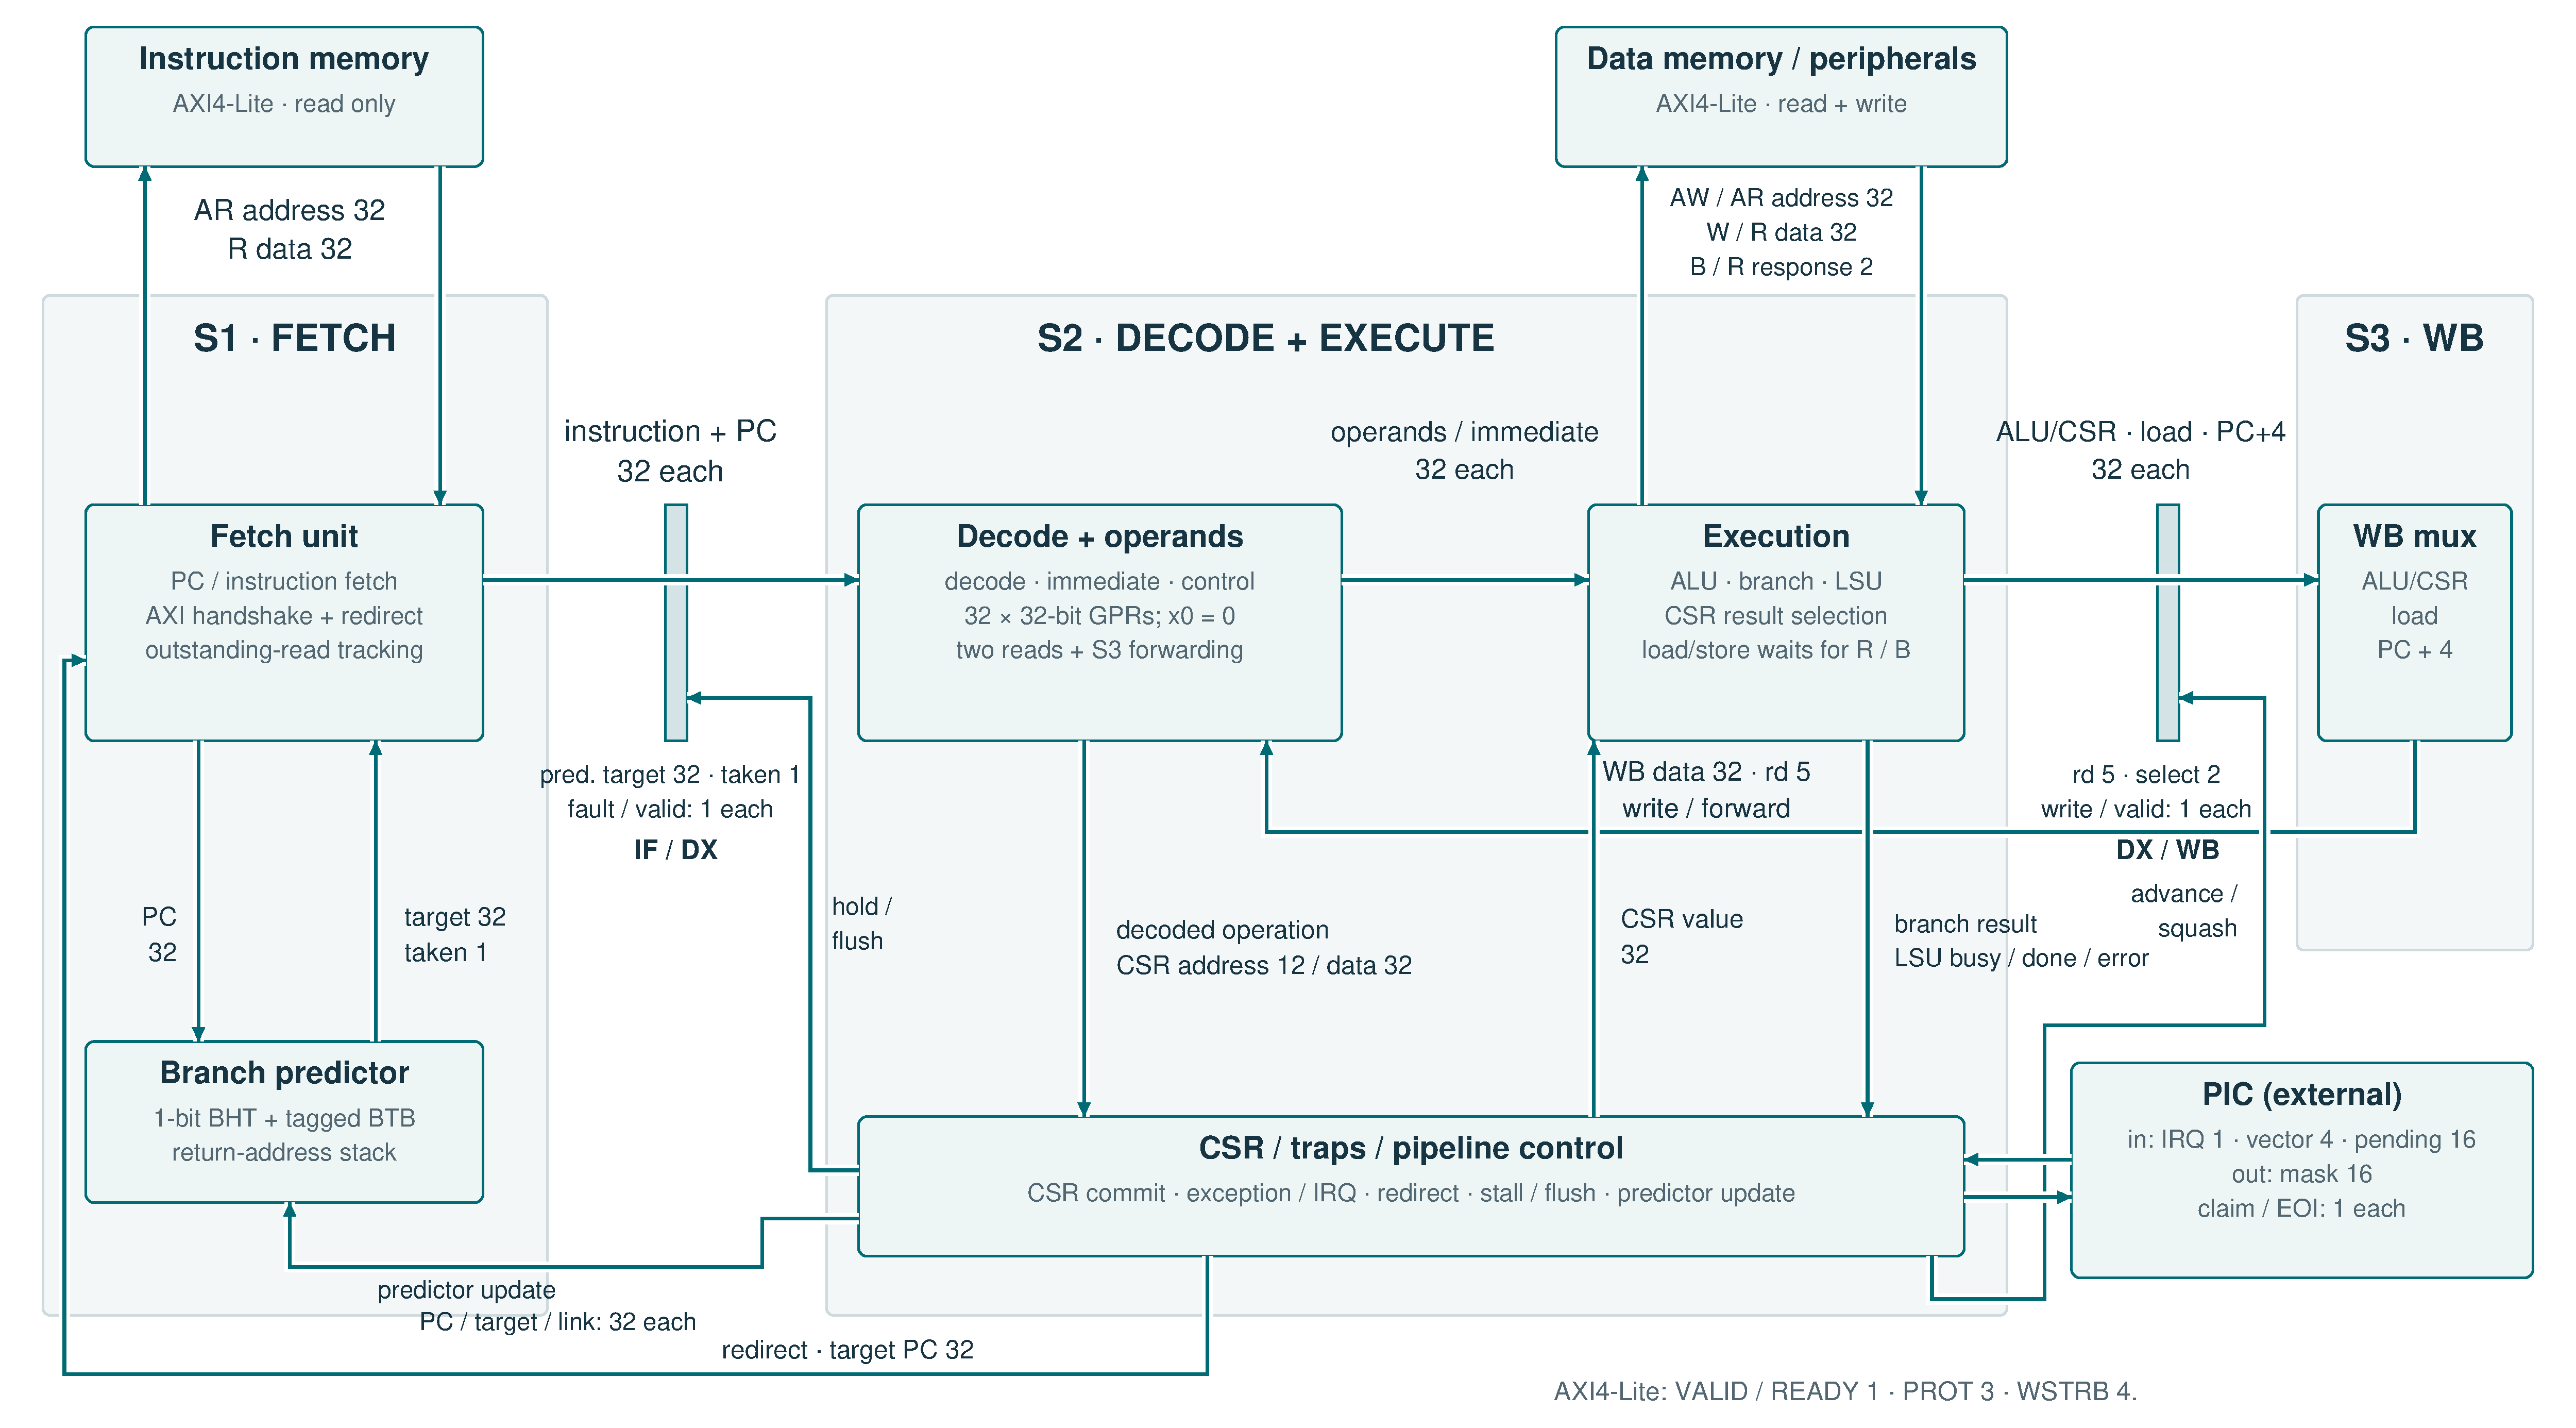
\includegraphics[width=\linewidth,height=132mm,keepaspectratio]{figures/cpu_essential.pdf}\caption{Three stages with pipeline boundaries, data paths and essential control feedback; widths are in bits. PIC and memories are external.}\end{figure}

\end{landscape}
\restoregeometry
\clearpage
\subsection{Pipeline and control contract}
\noindent Each stage owns one part of an instruction, and only S2 decides when an instruction is finished. The table states what each stage is responsible for, and which redirect wins when several are requested in the same cycle.\par\medskip
{\small
\begin{longtable}{@{}L{0.2200\dimexpr\linewidth-12pt\relax}L{0.7800\dimexpr\linewidth-12pt\relax}@{}}
\toprule
\textbf{Stage / control} & \textbf{Behaviour} \\ \midrule
\endfirsthead
\toprule
\textbf{Stage / control} & \textbf{Behaviour} \\ \midrule
\endhead
S1 & One outstanding instruction read; predictor selects next PC; wrong-path responses are drained and discarded. \\ \addlinespace[3pt]
S2 & Decode, execute and complete memory access. CSR side effects / instruction retirement occur at completion. \\ \addlinespace[3pt]
S3 & Write result to the destination GPR. Forward this value to dependent S2 operands. \\ \addlinespace[3pt]
Redirect priority & Synchronous trap / accepted interrupt, then MRET, then branch correction; redirect requires S2 to advance. \\ \addlinespace[3pt]
\bottomrule\end{longtable}}

\clearpage
\subsection{Instruction groups}
\noindent Integer instructions execute in order. Loads and stores complete in S2; CSR effects also commit there, while GPR writeback occurs in S3.\par\medskip
{\small
\begin{longtable}{@{}L{0.2800\dimexpr\linewidth-12pt\relax}L{0.7200\dimexpr\linewidth-12pt\relax}@{}}
\toprule
\textbf{Group} & \textbf{Implemented instructions / behavior} \\ \midrule
\endfirsthead
\toprule
\textbf{Group} & \textbf{Implemented instructions / behavior} \\ \midrule
\endhead
Arithmetic / upper immediate & ADD, ADDI, SUB, LUI, AUIPC. \\ \addlinespace[3pt]
Logic & AND/ANDI, OR/ORI, XOR/XORI. \\ \addlinespace[3pt]
Shift & SLL/SLLI, SRL/SRLI, SRA/SRAI. \\ \addlinespace[3pt]
Compare & SLT/SLTI, SLTU/SLTIU. \\ \addlinespace[3pt]
Control transfer & BEQ, BNE, BLT, BGE, BLTU, BGEU, JAL and JALR. \\ \addlinespace[3pt]
Load / store & LB, LH, LW, LBU, LHU; SB, SH, SW. Naturally aligned accesses only. \\ \addlinespace[3pt]
System & ECALL, EBREAK, FENCE as a no-op; CSRRW/CSRRS/CSRRC and immediate variants; MRET and WFI. \\ \addlinespace[3pt]
Unsupported encoding & Illegal-instruction exception, including M/A/C instructions and FENCE.I. \\ \addlinespace[3pt]
\bottomrule\end{longtable}}

\clearpage
\subsection{Branch prediction}
\noindent Prediction chooses the next fetch address; S2 remains responsible for resolving the instruction and committing any predictor update.\par\medskip
{\small
\begin{longtable}{@{}L{0.2500\dimexpr\linewidth-12pt\relax}L{0.7500\dimexpr\linewidth-12pt\relax}@{}}
\toprule
\textbf{Decision} & \textbf{Behaviour} \\ \midrule
\endfirsthead
\toprule
\textbf{Decision} & \textbf{Behaviour} \\ \midrule
\endhead
Table and mapping & BP\_ENTRIES=128 by default. A direct-mapped entry uses PC[IDX\_W+1:2], with IDX\_W=log2(BP\_ENTRIES); upper PC bits form the tag. An alias replaces that indexed entry. \\ \addlinespace[3pt]
Unseen branch & Invalid entry or tag miss predicts not taken, selecting PC+4. Each valid entry stores one direction bit and a 32-bit target. \\ \addlinespace[3pt]
Misprediction & At S2, compare predicted direction with the resolved direction; for a taken transfer also compare targets. A mismatch redirects fetch when S2 advances. \\ \addlinespace[3pt]
Update point & A live, non-faulting branch/jump updates direction, tag and target at S2 completion, including the correcting edge. Wrong-path or trapping instructions do not train the table. \\ \addlinespace[3pt]
Trap entry / return & BTB/BHT and RAS are preserved across traps and MRET; reset clears them. \\ \addlinespace[3pt]
Call / return & RAS\_DEPTH=8 by default; zero disables the stack. JAL/JALR hints use x1/x5. Return entries use the stack top, falling back to the BTB target when empty. Full pushes replace the oldest entry; empty pops have no effect. \\ \addlinespace[3pt]
\bottomrule\end{longtable}}

\clearpage
\subsection{Trap entry, return and competing events}
\noindent Trap acceptance cancels the current S2 instruction and redirects younger fetch work. Older S3 work can still complete; the saved PC identifies where software must resume.\par\medskip
{\small
\begin{longtable}{@{}L{0.2500\dimexpr\linewidth-12pt\relax}L{0.7500\dimexpr\linewidth-12pt\relax}@{}}
\toprule
\textbf{Decision} & \textbf{Behaviour} \\ \midrule
\endfirsthead
\toprule
\textbf{Decision} & \textbf{Behaviour} \\ \midrule
\endhead
Entry edge & When trap\_take and s2\_advance are true, save mepc/mcause/mtval, copy MIE to MPIE, clear MIE, invalidate the incoming IF/DX entry and suppress the S2-to-S3 valid bit. \\ \addlinespace[3pt]
Return PC & Synchronous exceptions save the faulting instruction PC. An ordinary interrupt saves the preempted S2 PC. An interrupt accepted at WFI saves PC+4; software advances mepc when it elects to skip a synchronous fault. \\ \addlinespace[3pt]
Competing redirect & An eligible interrupt preempts the current instruction before synchronous exception evaluation. Otherwise a synchronous exception wins over MRET and branch correction. Redirect requires S2 completion. \\ \addlinespace[3pt]
Data transfer in progress & lsu\_active prevents IRQ acceptance until the outstanding access completes. An error response causes the load/store access-fault exception at completion. \\ \addlinespace[3pt]
Nested service & Trap entry clears MIE. Software must save trap CSRs and handler context before enabling nested interrupts. A 16-level trap-kind stack distinguishes interrupt returns from exception returns; software must keep combined depth at or below 16. \\ \addlinespace[3pt]
MRET & Restore MIE from MPIE, set MPIE, redirect to mepc and pop one trap level. Emit EOI only if the popped level was an interrupt; cpu\_in\_trap remains high while any level is open. \\ \addlinespace[3pt]
MIE write versus IRQ & Arbitration uses the current MIE value. With MIE=0, a CSR write enabling it completes before later acceptance. With MIE=1 and an eligible offer, IRQ preempts the CSR instruction; that instruction can execute after return. \\ \addlinespace[3pt]
WFI & Hold S2 until a locally enabled offer exists. Wakeup does not require global MIE; entering the interrupt handler does. \\ \addlinespace[3pt]
\bottomrule\end{longtable}}

\clearpage
\subsection{Stall, forwarding and flush}
\noindent Centralized pipeline control decides advancement and invalidation. A stalled memory instruction holds its operands in S2 while S3 receives bubbles after older work completes.\par\medskip
{\small
\begin{longtable}{@{}L{0.2500\dimexpr\linewidth-12pt\relax}L{0.7500\dimexpr\linewidth-12pt\relax}@{}}
\toprule
\textbf{Decision} & \textbf{Behaviour} \\ \midrule
\endfirsthead
\toprule
\textbf{Decision} & \textbf{Behaviour} \\ \midrule
\endhead
Fetch unavailable & No fetched instruction inserts an IF/DX bubble when S2 can advance. Fetch tracks its own address/response and may retain one returned instruction while S2 is stalled. \\ \addlinespace[3pt]
Data access / WFI & lsu\_busy or wfi\_wait holds IF/DX. S3 valid is cleared while S2 is held, preventing repeated writeback. \\ \addlinespace[3pt]
Load-use dependency & S2 waits for the load response. Once the load reaches S3, its result forwards to either matching S2 operand; no extra load-use bubble is needed. x0 is excluded from forwarding. \\ \addlinespace[3pt]
Stall and redirect & A redirect is gated by s2\_advance, so the active data access completes first. At the advancing edge, trap/MRET/correction determines the new fetch address and IF/DX receives a bubble. \\ \addlinespace[3pt]
Wrong-path fetch & An accepted AR cannot be cancelled. An outstanding wrong-path response is drained and discarded; it cannot create a GPR write or instruction-access exception. \\ \addlinespace[3pt]
Pipeline registers & IF/DX stores instruction, PC, prediction and fault with valid. DX/WB stores the destination and result choices with valid. Reset clears valid bits and initializes the instruction to ADDI x0,x0,0; invalid payloads cannot execute. \\ \addlinespace[3pt]
\bottomrule\end{longtable}}

\clearpage
\subsection{Independent memory ports}
\noindent Instruction fetch and the LSU have separate AXI channel state. They can progress concurrently; the pipeline consumes their results in order.\par\medskip
{\small
\begin{longtable}{@{}L{0.2500\dimexpr\linewidth-12pt\relax}L{0.7500\dimexpr\linewidth-12pt\relax}@{}}
\toprule
\textbf{Decision} & \textbf{Behaviour} \\ \midrule
\endfirsthead
\toprule
\textbf{Decision} & \textbf{Behaviour} \\ \midrule
\endhead
Both ports stalled & Hold each VALID and payload until its own READY. S2 retains the data operation; a fetched instruction can be held until S2 becomes available. \\ \addlinespace[3pt]
Read / write errors & Instruction RRESP[1] becomes instruction-access fault (cause 1). Data RRESP[1]/BRESP[1] becomes load/store access fault (5/7); the faulting instruction cannot write its destination. \\ \addlinespace[3pt]
Future AXI4 integration & An external Lite-to-Full wrapper can emit single-beat transactions with fixed ID, LEN=0, SIZE=2 and no outstanding reordering. Bursts or multiple outstanding instructions would require new request tracking and verification; the current CPU ports remain AXI4-Lite. \\ \addlinespace[3pt]
\bottomrule\end{longtable}}

\clearpage
\section{Interfaces}
\subsection{Hardware interface}
\noindent The two memory ports and PIC link are independent interfaces on the same clock domain. Capacity parameters do not change their external bus widths.\par\medskip
{\small
\begin{longtable}{@{}L{0.2500\dimexpr\linewidth-24pt\relax}L{0.2300\dimexpr\linewidth-24pt\relax}L{0.5200\dimexpr\linewidth-24pt\relax}@{}}
\toprule
\textbf{Parameter} & \textbf{Default} & \textbf{Meaning / valid setting} \\ \midrule
\endfirsthead
\toprule
\textbf{Parameter} & \textbf{Default} & \textbf{Meaning / valid setting} \\ \midrule
\endhead
RESET\_PC & 32'h0000\_0000 & Word-aligned first fetch address. \\ \addlinespace[3pt]
HART\_ID & 32'd0 & Value returned by mhartid. \\ \addlinespace[3pt]
BP\_ENTRIES & 128 & BTB/BHT entries; power of two, at least 2. \\ \addlinespace[3pt]
RAS\_DEPTH & 8 & Return-address stack entries; zero disables it. \\ \addlinespace[3pt]
\bottomrule\end{longtable}}
{\small
\begin{longtable}{@{}L{0.2600\dimexpr\linewidth-12pt\relax}L{0.7400\dimexpr\linewidth-12pt\relax}@{}}
\toprule
\textbf{Width class} & \textbf{Contract} \\ \midrule
\endfirsthead
\toprule
\textbf{Width class} & \textbf{Contract} \\ \midrule
\endhead
Architectural widths & Instructions, addresses and data are fixed at 32 bits; GPR indices are 5 bits. \\ \addlinespace[3pt]
Interrupt widths & 16 mask/pending bits, 4-bit source ID. These are fixed widths, not module parameters. \\ \addlinespace[3pt]
Prediction capacity & BP\_ENTRIES and RAS\_DEPTH change internal capacity, not external bus widths. \\ \addlinespace[3pt]
\bottomrule\end{longtable}}
{\small
\begin{longtable}{@{}L{0.3400\dimexpr\linewidth-36pt\relax}L{0.1000\dimexpr\linewidth-36pt\relax}L{0.1000\dimexpr\linewidth-36pt\relax}L{0.4600\dimexpr\linewidth-36pt\relax}@{}}
\toprule
\textbf{Signal} & \textbf{Dir.} & \textbf{Width (bits)} & \textbf{Meaning} \\ \midrule
\endfirsthead
\toprule
\textbf{Signal} & \textbf{Dir.} & \textbf{Width (bits)} & \textbf{Meaning} \\ \midrule
\endhead
\texttt{clk\_i} & input & 1 & Rising-edge clock input. \\ \addlinespace[3pt]
\texttt{rst\_n\_i} & input & 1 & Asynchronous reset, active low. \\ \addlinespace[3pt]
\texttt{ibus\_axi\_araddr\_o} & output & 32 & Read byte address. \\ \addlinespace[3pt]
\texttt{ibus\_axi\_arprot\_o} & output & 3 & Read protection attributes. \\ \addlinespace[3pt]
\texttt{ibus\_axi\_arvalid\_o} & output & 1 & Read address is valid; hold until handshake. \\ \addlinespace[3pt]
\texttt{ibus\_axi\_arready\_i} & input & 1 & Receiver can accept the read address. \\ \addlinespace[3pt]
\texttt{ibus\_axi\_rdata\_i} & input & 32 & Read payload. \\ \addlinespace[3pt]
\texttt{ibus\_axi\_rresp\_i} & input & 2 & Read response: OKAY=00, SLVERR=10, DECERR=11. \\ \addlinespace[3pt]
\texttt{ibus\_axi\_rvalid\_i} & input & 1 & Read response is valid; hold until handshake. \\ \addlinespace[3pt]
\texttt{ibus\_axi\_rready\_o} & output & 1 & Receiver can accept the read response. \\ \addlinespace[3pt]
\texttt{dbus\_axi\_awaddr\_o} & output & 32 & Write byte address. \\ \addlinespace[3pt]
\texttt{dbus\_axi\_awprot\_o} & output & 3 & Write protection attributes. \\ \addlinespace[3pt]
\texttt{dbus\_axi\_awvalid\_o} & output & 1 & Write address is valid; hold until handshake. \\ \addlinespace[3pt]
\texttt{dbus\_axi\_awready\_i} & input & 1 & Receiver can accept the write address. \\ \addlinespace[3pt]
\texttt{dbus\_axi\_wdata\_o} & output & 32 & Write payload. \\ \addlinespace[3pt]
\texttt{dbus\_axi\_wstrb\_o} & output & 4 & One enable bit per write byte. \\ \addlinespace[3pt]
\texttt{dbus\_axi\_wvalid\_o} & output & 1 & Write data is valid; hold until handshake. \\ \addlinespace[3pt]
\texttt{dbus\_axi\_wready\_i} & input & 1 & Receiver can accept the write data. \\ \addlinespace[3pt]
\texttt{dbus\_axi\_bresp\_i} & input & 2 & Write response: OKAY=00, SLVERR=10, DECERR=11. \\ \addlinespace[3pt]
\texttt{dbus\_axi\_bvalid\_i} & input & 1 & Write response is valid; hold until handshake. \\ \addlinespace[3pt]
\texttt{dbus\_axi\_bready\_o} & output & 1 & Receiver can accept the write response. \\ \addlinespace[3pt]
\texttt{dbus\_axi\_araddr\_o} & output & 32 & Read byte address. \\ \addlinespace[3pt]
\texttt{dbus\_axi\_arprot\_o} & output & 3 & Read protection attributes. \\ \addlinespace[3pt]
\texttt{dbus\_axi\_arvalid\_o} & output & 1 & Read address is valid; hold until handshake. \\ \addlinespace[3pt]
\texttt{dbus\_axi\_arready\_i} & input & 1 & Receiver can accept the read address. \\ \addlinespace[3pt]
\texttt{dbus\_axi\_rdata\_i} & input & 32 & Read payload. \\ \addlinespace[3pt]
\texttt{dbus\_axi\_rresp\_i} & input & 2 & Read response: OKAY=00, SLVERR=10, DECERR=11. \\ \addlinespace[3pt]
\texttt{dbus\_axi\_rvalid\_i} & input & 1 & Read response is valid; hold until handshake. \\ \addlinespace[3pt]
\texttt{dbus\_axi\_rready\_o} & output & 1 & Receiver can accept the read response. \\ \addlinespace[3pt]
\texttt{cpu\_irq\_i} & input & 1 & Prioritized interrupt request from PIC. \\ \addlinespace[3pt]
\texttt{cpu\_irq\_vec\_i} & input & 4 & Source ID associated with cpu\_irq\_i. \\ \addlinespace[3pt]
\texttt{irq\_pending\_i} & input & 16 & Enabled pending sources from PIC; exposed in mip[31:16]. \\ \addlinespace[3pt]
\texttt{irq\_mask\_o} & output & 16 & mie[31:16], sent to the PIC resolver. \\ \addlinespace[3pt]
\texttt{cpu\_irq\_ack\_o} & output & 1 & Registered one-cycle claim to PIC. \\ \addlinespace[3pt]
\texttt{cpu\_irq\_eoi\_o} & output & 1 & One-cycle EOI on return from an interrupt. \\ \addlinespace[3pt]
\texttt{cpu\_in\_trap\_o} & output & 1 & CPU has an active trap context. \\ \addlinespace[3pt]
\bottomrule\end{longtable}}

\clearpage
\subsubsection{Reset contract}
\noindent Reset must leave the core in a state software can start from, without needing a clock edge to get there. The table lists what reset forces; the waveform below shows it interrupting a fetch that is already in progress.\par\medskip
{\small
\begin{longtable}{@{}L{0.2500\dimexpr\linewidth-12pt\relax}L{0.7500\dimexpr\linewidth-12pt\relax}@{}}
\toprule
\textbf{Item} & \textbf{Required behaviour} \\ \midrule
\endfirsthead
\toprule
\textbf{Item} & \textbf{Required behaviour} \\ \midrule
\endhead
Clock & Sequential state updates on posedge clk\_i. \\ \addlinespace[3pt]
Assertion & Asynchronous active-low rst\_n\_i; no clock edge required for assertion. \\ \addlinespace[3pt]
Outputs & AXI request VALID signals, IRQ claim/EOI and trap-active state are inactive. \\ \addlinespace[3pt]
Architectural state & GPRs=0; PC=RESET\_PC; mstatus=0x1800; other stored CSRs/counters=0, except documented fixed values. \\ \addlinespace[3pt]
mip & Combinational pending input, not a reset storage element. Zero requires irq\_pending\_i=0. \\ \addlinespace[3pt]
Integration & Distribute reset to CPU and bus responders. Release it with the system reset controller; release between clock edges is also supported. \\ \addlinespace[3pt]
\bottomrule\end{longtable}}

\noindent Reset is asserted while an instruction request is waiting. ARVALID clears at the reset event, before the next rising edge; after release the fetch request resumes from RESET\_PC.\par
\begin{figure}[H]\centering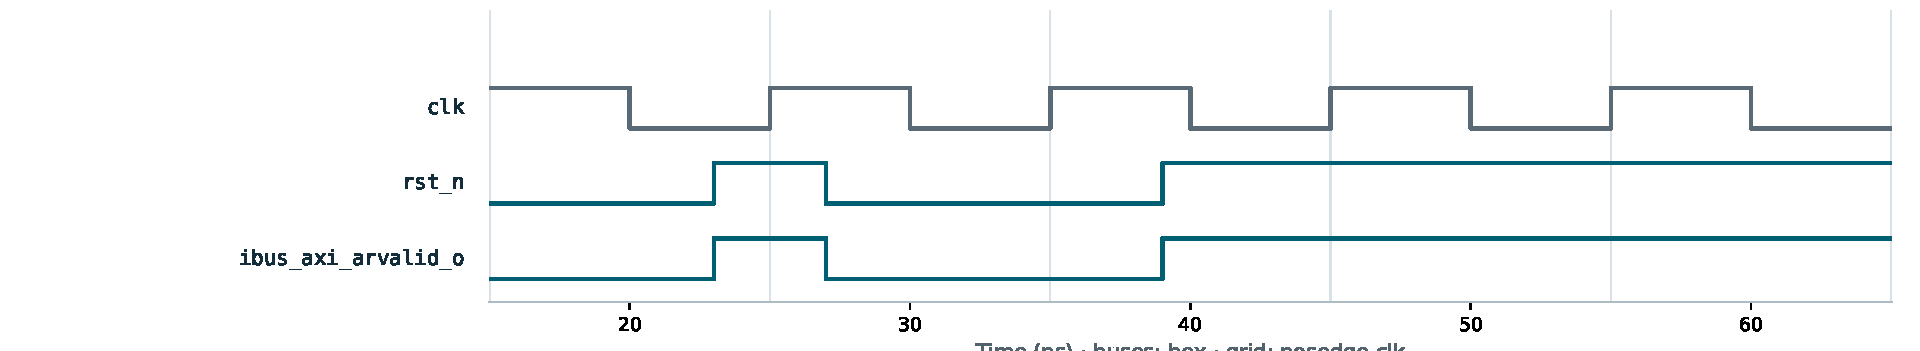
\includegraphics[width=\linewidth]{waves/cpu_reset.pdf}\caption{Instruction request interrupted by asynchronous reset at 27 ns.}\end{figure}

\clearpage
\subsubsection{Instruction AXI4-Lite interface}

\noindent ARVALID remains asserted until the instruction address is accepted. The R handshake supplies the instruction to IF/DX; the address trace shows the next sequential fetch.\par
\begin{figure}[H]\centering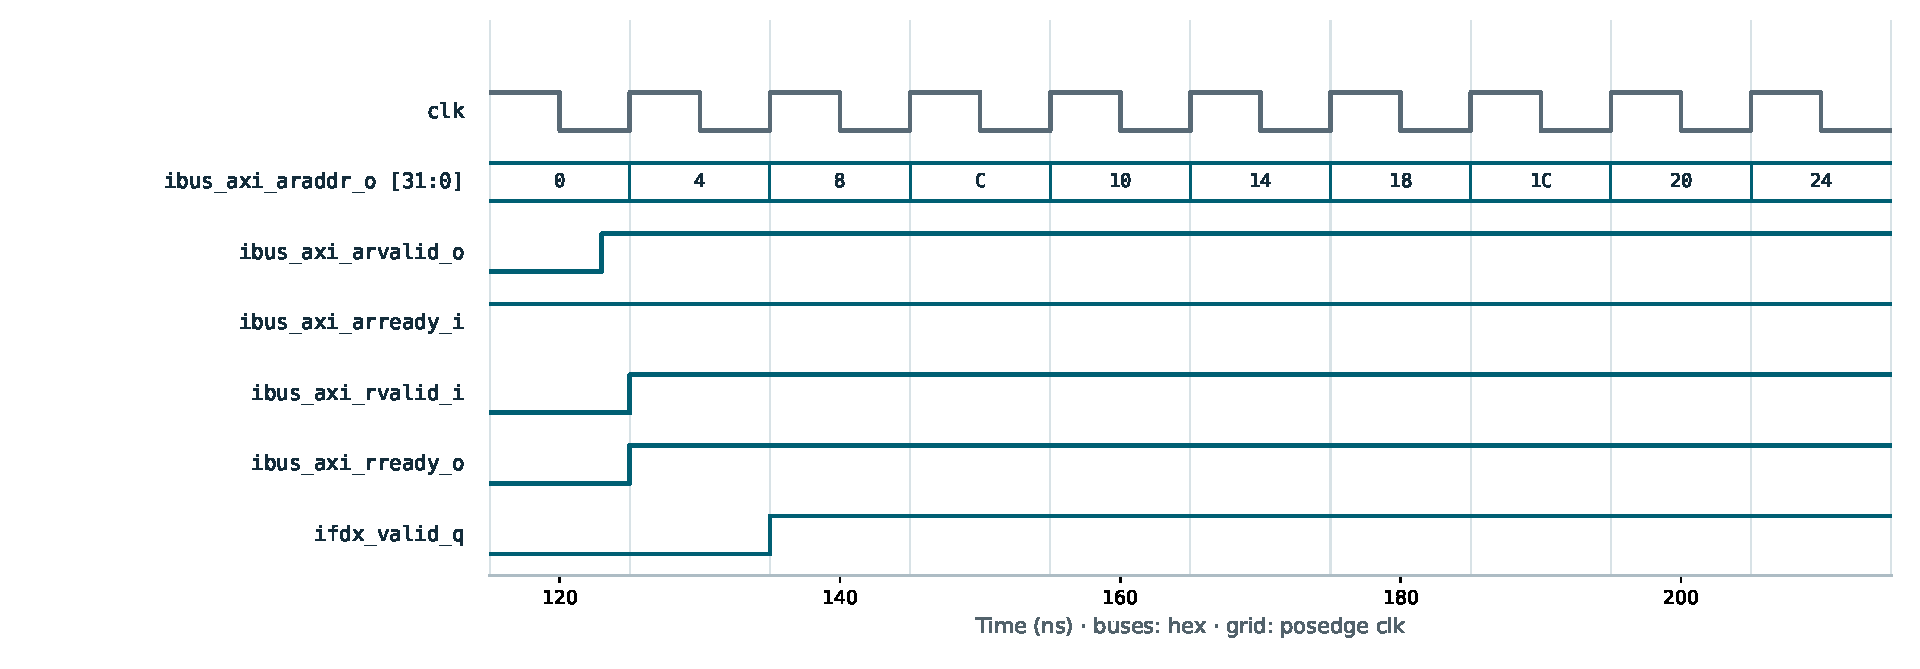
\includegraphics[width=\linewidth]{waves/cpu_fetch.pdf}\caption{Instruction fetch after rst\_n release at 123 ns.}\end{figure}
{\small
\begin{longtable}{@{}L{0.2500\dimexpr\linewidth-12pt\relax}L{0.7500\dimexpr\linewidth-12pt\relax}@{}}
\toprule
\textbf{Property} & \textbf{Contract} \\ \midrule
\endfirsthead
\toprule
\textbf{Property} & \textbf{Contract} \\ \midrule
\endhead
Channels & AR/R only; fixed 32-bit address and data. \\ \addlinespace[3pt]
Handshake & Transfer at posedge when VALID and READY are both high; retain VALID and payload while stalled. \\ \addlinespace[3pt]
Outstanding requests & At most one; issuing the next AR may overlap completion of the prior R. \\ \addlinespace[3pt]
Protection & ARPROT=111: instruction, non-secure, privileged. \\ \addlinespace[3pt]
Errors & SLVERR/DECERR become an instruction-access fault in S2. A wrong-path fault is discarded. \\ \addlinespace[3pt]
Redirect & An accepted request cannot be cancelled. Retain its route / drain the response before using the new path. \\ \addlinespace[3pt]
\bottomrule\end{longtable}}

\clearpage
\subsubsection{Data AXI4-Lite interface}

\noindent The load holds S2 while its request or response is pending. At the RVALID/RREADY handshake, the data is available and s2\_advance permits the instruction to enter writeback.\par
\begin{figure}[H]\centering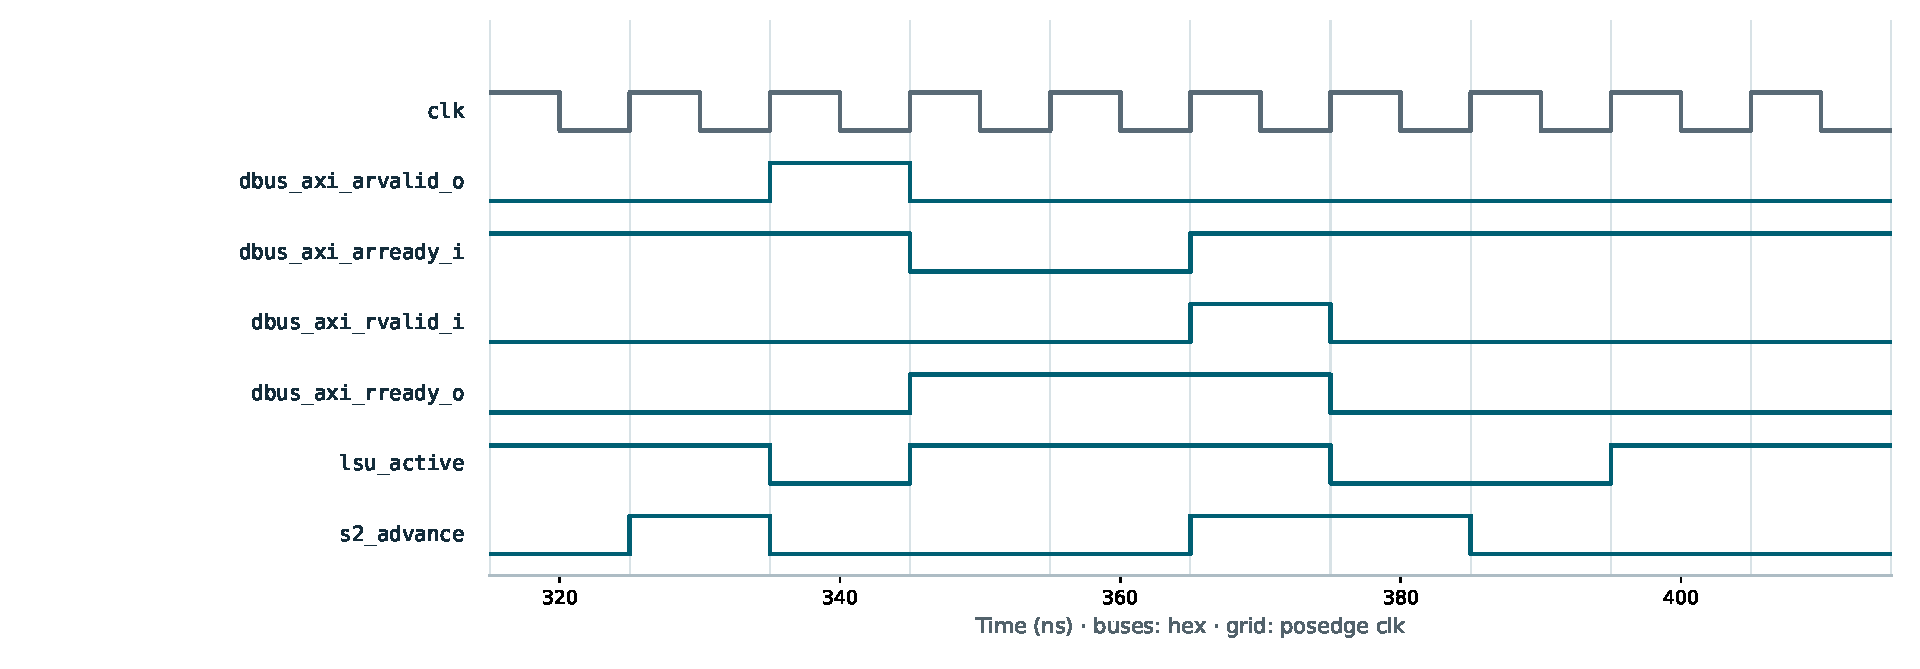
\includegraphics[width=\linewidth]{waves/cpu_load.pdf}\caption{Load: lsu\_active holds S2 until the data response completes.}\end{figure}

\noindent AW and W are accepted independently. The store completes only when the B response is accepted, so an earlier address or data handshake alone does not release the instruction.\par
\begin{figure}[H]\centering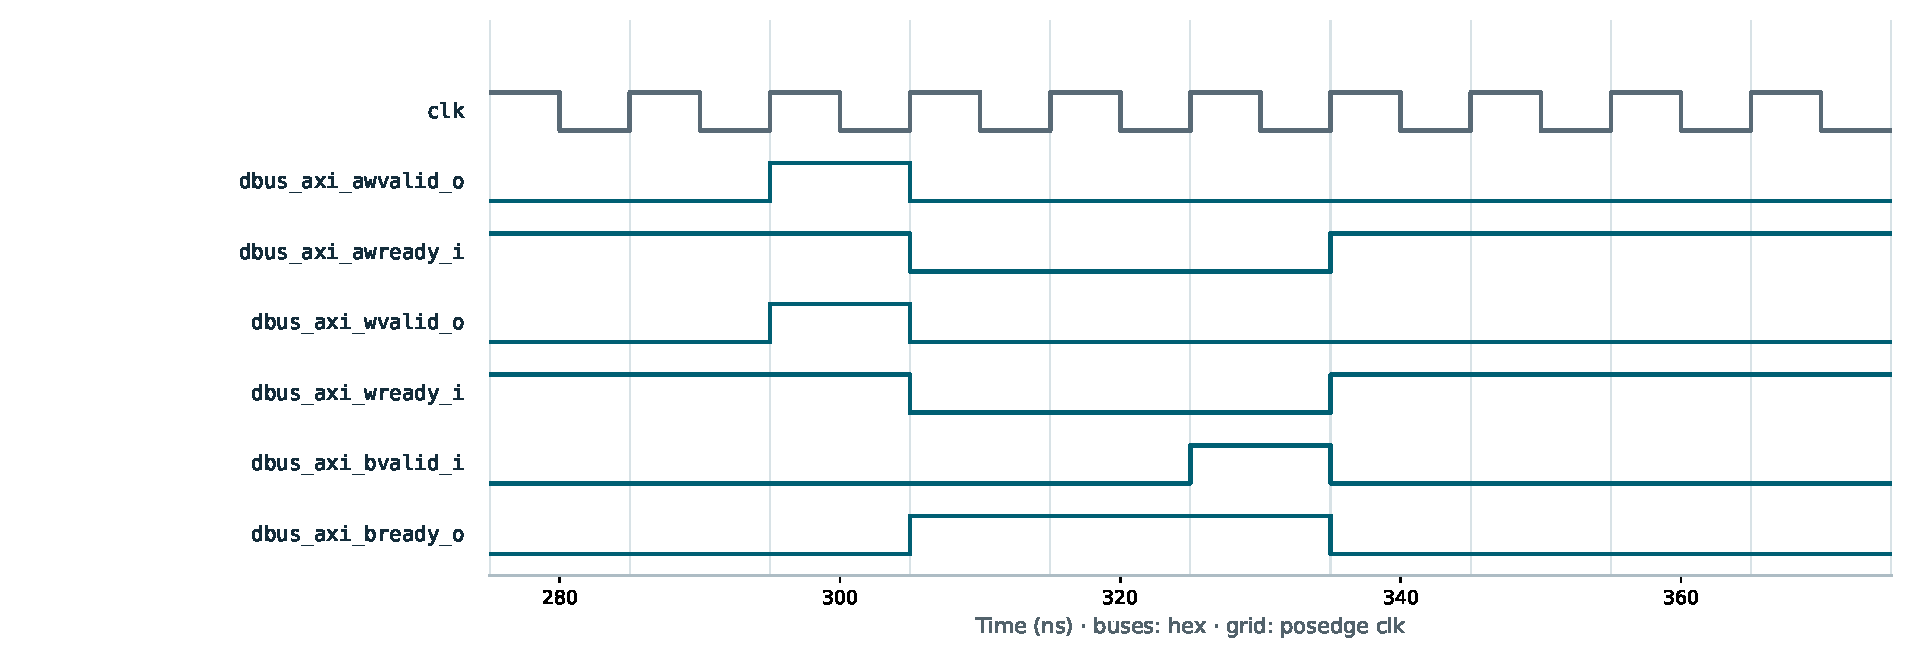
\includegraphics[width=\linewidth]{waves/cpu_store.pdf}\caption{Store: address and write data are accepted independently; B completes the store.}\end{figure}
{\small
\begin{longtable}{@{}L{0.2400\dimexpr\linewidth-12pt\relax}L{0.7600\dimexpr\linewidth-12pt\relax}@{}}
\toprule
\textbf{Property} & \textbf{Contract} \\ \midrule
\endfirsthead
\toprule
\textbf{Property} & \textbf{Contract} \\ \midrule
\endhead
Transactions & One load or store outstanding; byte, halfword and word accesses. \\ \addlinespace[3pt]
Byte lanes & WSTRB selects bytes; reads extract/sign-extend according to the instruction. \\ \addlinespace[3pt]
Misalignment & Detected before bus issue; misaligned accesses trap. \\ \addlinespace[3pt]
Errors & SLVERR/DECERR produce load/store access faults; destination is not committed. \\ \addlinespace[3pt]
Protection & AWPROT/ARPROT=011: data, non-secure, privileged. \\ \addlinespace[3pt]
\bottomrule\end{longtable}}

\clearpage
\subsubsection{Interrupts and redirects}

\noindent The interrupt arrives while the LSU is active. Marker 2 identifies the accepted load response; marker 3 shows the registered claim and trap-active state at the next instruction boundary.\par
\begin{figure}[H]\centering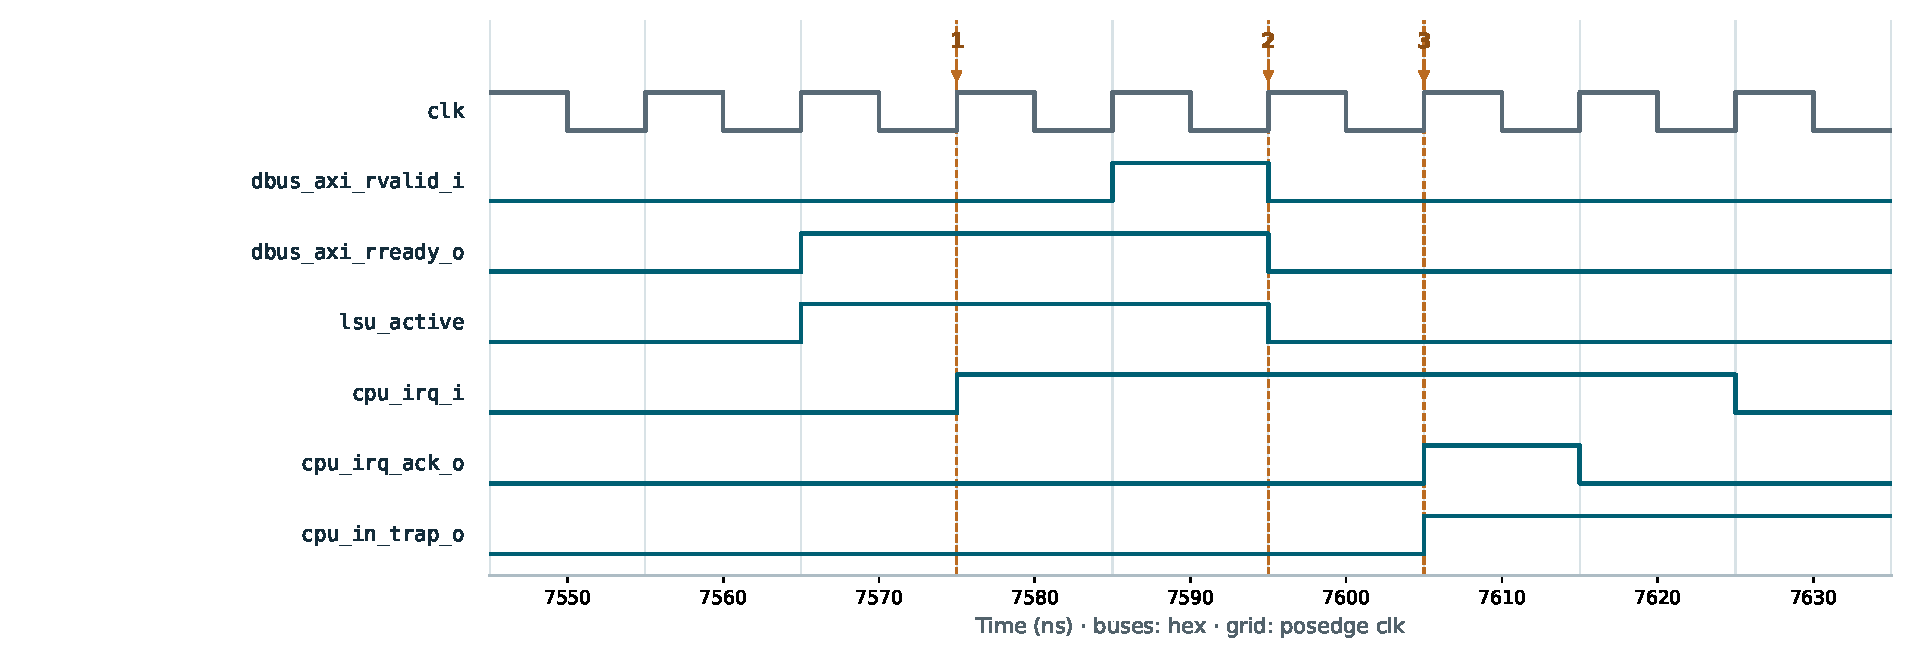
\includegraphics[width=\linewidth]{waves/cpu_irq.pdf}\caption{Interrupt claim: cpu\_irq\_ack\_o is a full-cycle registered pulse.}\end{figure}

\noindent The resolved branch differs from the prediction, causing redirect. IF/DX is invalidated so younger work cannot commit; an outstanding fetch response still completes its AXI transaction.\par
\begin{figure}[H]\centering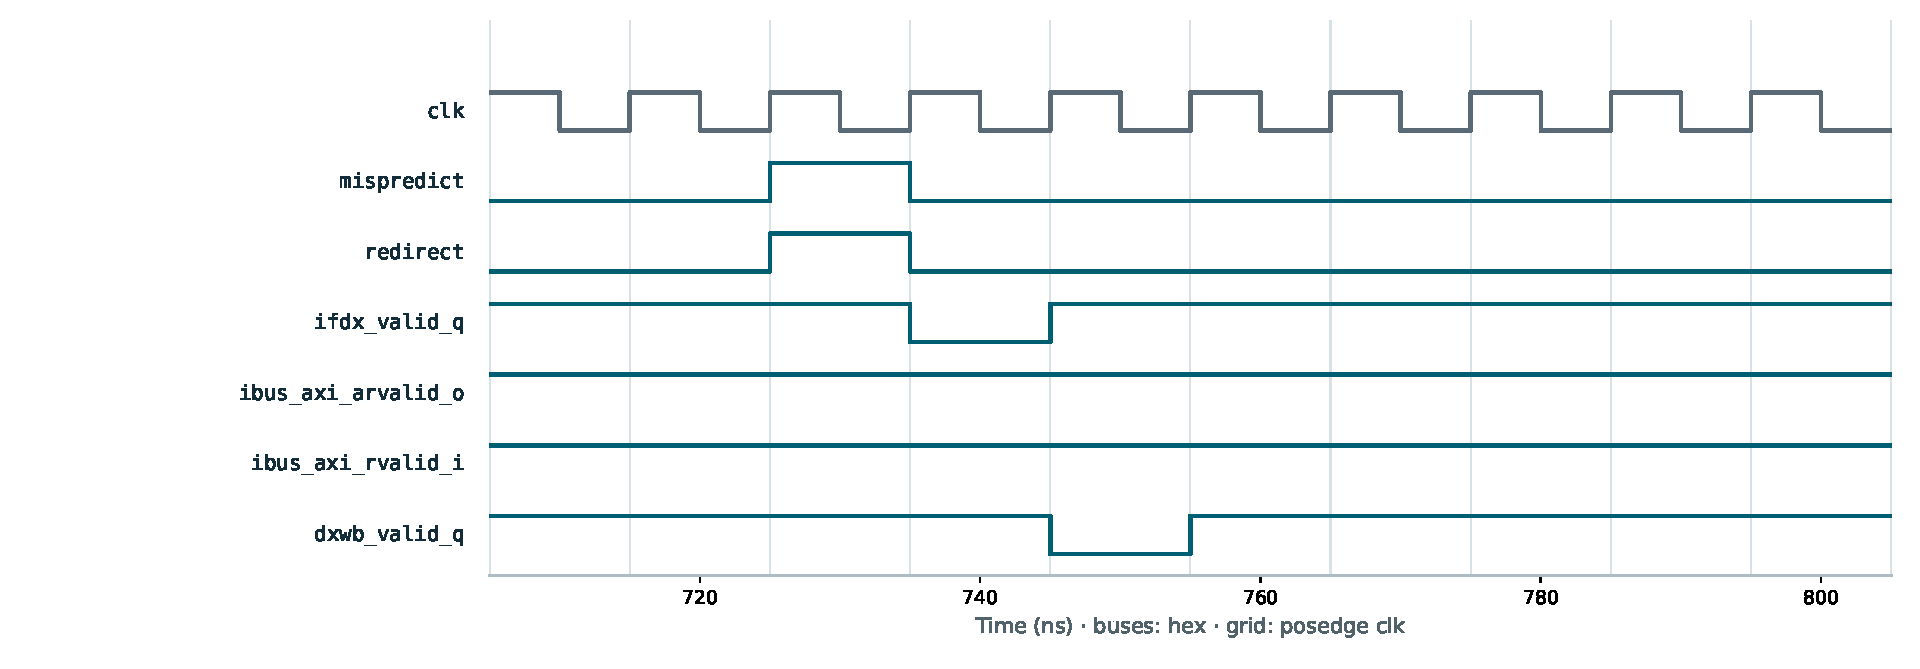
\includegraphics[width=\linewidth]{waves/cpu_redirect.pdf}\caption{Branch correction: redirect invalidates younger work.}\end{figure}
{\small
\begin{longtable}{@{}L{0.2400\dimexpr\linewidth-12pt\relax}L{0.7600\dimexpr\linewidth-12pt\relax}@{}}
\toprule
\textbf{Event} & \textbf{Contract} \\ \midrule
\endfirsthead
\toprule
\textbf{Event} & \textbf{Contract} \\ \midrule
\endhead
Interrupt eligibility & mstatus.MIE and the enabled source must allow it; acceptance waits for an instruction boundary, including completion of an active LSU transfer. \\ \addlinespace[3pt]
Cause & External source n uses mcause=0x80000000 | (16+n). \\ \addlinespace[3pt]
Claim / EOI & Claim is sent after the offer is sampled. EOI is sent when returning from an interrupt; a synchronous exception return does not pop the PIC. \\ \addlinespace[3pt]
Nested software & Save mepc, mstatus and handler context before enabling nested interrupts; restore before MRET. \\ \addlinespace[3pt]
\bottomrule\end{longtable}}

\clearpage
\subsection{Software interface}
\noindent The CSR file is the only software-visible interface of the core, and it is reached through CSR instructions rather than through the AXI ports. The map lists every implemented address with its access class and reset value; the subsections that follow give the fields of each register.\par\medskip
{\small
\begin{longtable}{@{}L{0.1900\dimexpr\linewidth-48pt\relax}L{0.2300\dimexpr\linewidth-48pt\relax}L{0.1400\dimexpr\linewidth-48pt\relax}L{0.1500\dimexpr\linewidth-48pt\relax}L{0.2900\dimexpr\linewidth-48pt\relax}@{}}
\toprule
\textbf{Address} & \textbf{Name} & \textbf{Access type} & \textbf{Reset} & \textbf{Description} \\ \midrule
\endfirsthead
\toprule
\textbf{Address} & \textbf{Name} & \textbf{Access type} & \textbf{Reset} & \textbf{Description} \\ \midrule
\endhead
0x300 & mstatus & RW / fixed & 0x00001800 & Global interrupt state. \\ \addlinespace[3pt]
0x301 & misa & WARL / fixed & 0x40000100 & RV32I capability. \\ \addlinespace[3pt]
0x304 & mie & RW & 0 & Interrupt enables [31:16]. \\ \addlinespace[3pt]
0x305 & mtvec & RW / WARL & 0 & Trap base and mode. \\ \addlinespace[3pt]
0x323–0x327 & mhpmevent3..7 & WARL / fixed & 1..5 & Fixed performance-event selectors. \\ \addlinespace[3pt]
0x328–0x33F & mhpmevent8..31 & WARL / fixed & 0 & Unused event selectors. \\ \addlinespace[3pt]
0x340 & mscratch & RW & 0 & Software scratch word. \\ \addlinespace[3pt]
0x341 & mepc & RW / aligned & 0 & Trap return PC. \\ \addlinespace[3pt]
0x342 & mcause & RW & 0 & Trap cause. \\ \addlinespace[3pt]
0x343 & mtval & RW & 0 & Fault payload. \\ \addlinespace[3pt]
0x344 & mip & RO & input-dependent & irq\_pending\_i in [31:16]. \\ \addlinespace[3pt]
0xB00 / 0xB80 & mcycle / mcycleh & RW & 0 & 64-bit cycle count. \\ \addlinespace[3pt]
0xB02 / 0xB82 & minstret / minstreth & RW & 0 & 64-bit completed-instruction count. \\ \addlinespace[3pt]
0xB03–0xB07 / 0xB83–0xB87 & mhpmcounter3..7 / high & RW & 0 & 64-bit event counts. \\ \addlinespace[3pt]
0xB08–0xB1F / 0xB88–0xB9F & mhpmcounter8..31 / high & WARL / fixed & 0 & Unused counters; writes ignored. \\ \addlinespace[3pt]
0xF11–0xF13 & mvendorid / marchid / mimpid & RO & 0 & Identification values. \\ \addlinespace[3pt]
0xF14 & mhartid & RO & HART\_ID & Instance identifier. \\ \addlinespace[3pt]
\bottomrule\end{longtable}}
{\small
\begin{longtable}{@{}L{0.3400\dimexpr\linewidth-12pt\relax}L{0.6600\dimexpr\linewidth-12pt\relax}@{}}
\toprule
\textbf{Access rule} & \textbf{Behaviour} \\ \midrule
\endfirsthead
\toprule
\textbf{Access rule} & \textbf{Behaviour} \\ \midrule
\endhead
Unknown address / read-only write & Illegal-instruction exception; CSR addresses are not memory-mapped AXI addresses. \\ \addlinespace[3pt]
CSRRW / CSRRS / CSRRC & Replace / set / clear; immediate variants use zero-extended zimm. Zero-source CSRRS/CSRRC do not write. \\ \addlinespace[3pt]
Unimplemented inhibit & 0x320 (mcountinhibit) is absent and traps. \\ \addlinespace[3pt]
\bottomrule\end{longtable}}

\clearpage
\subsubsection{CSR fields: status and interrupt enables}
\subsection*{mstatus — 0x300}
{\small
\begin{longtable}{@{}L{0.1200\dimexpr\linewidth-48pt\relax}L{0.1800\dimexpr\linewidth-48pt\relax}L{0.1200\dimexpr\linewidth-48pt\relax}L{0.1200\dimexpr\linewidth-48pt\relax}L{0.4600\dimexpr\linewidth-48pt\relax}@{}}
\toprule
\textbf{Bits} & \textbf{Field} & \textbf{Access type} & \textbf{Reset} & \textbf{Description} \\ \midrule
\endfirsthead
\toprule
\textbf{Bits} & \textbf{Field} & \textbf{Access type} & \textbf{Reset} & \textbf{Description} \\ \midrule
\endhead
[31:13], [10:8], [6:4], [2:0] & Reserved & RAZ/WI & 0 & Reads zero; writes ignored. \\ \addlinespace[3pt]
[12:11] & MPP & fixed & 3 & Machine mode only. \\ \addlinespace[3pt]
[7] & MPIE & RW + HW & 0 & Saved MIE; MRET sets it to 1. \\ \addlinespace[3pt]
[3] & MIE & RW + HW & 0 & Global enable; trap clears it; MRET restores MPIE. \\ \addlinespace[3pt]
\bottomrule\end{longtable}}
\subsection*{mie — 0x304}
{\small
\begin{longtable}{@{}L{0.1200\dimexpr\linewidth-48pt\relax}L{0.1800\dimexpr\linewidth-48pt\relax}L{0.1200\dimexpr\linewidth-48pt\relax}L{0.1200\dimexpr\linewidth-48pt\relax}L{0.4600\dimexpr\linewidth-48pt\relax}@{}}
\toprule
\textbf{Bits} & \textbf{Field} & \textbf{Access type} & \textbf{Reset} & \textbf{Description} \\ \midrule
\endfirsthead
\toprule
\textbf{Bits} & \textbf{Field} & \textbf{Access type} & \textbf{Reset} & \textbf{Description} \\ \midrule
\endhead
[31:16] & ENABLE & RW & 0 & 16 source-enable bits; exported as irq\_mask\_o. \\ \addlinespace[3pt]
[15:0] & Reserved & RAZ/WI & 0 & Reads zero; writes ignored. \\ \addlinespace[3pt]
\bottomrule\end{longtable}}
\subsection*{mip — 0x344}
{\small
\begin{longtable}{@{}L{0.1200\dimexpr\linewidth-48pt\relax}L{0.1800\dimexpr\linewidth-48pt\relax}L{0.1200\dimexpr\linewidth-48pt\relax}L{0.1200\dimexpr\linewidth-48pt\relax}L{0.4600\dimexpr\linewidth-48pt\relax}@{}}
\toprule
\textbf{Bits} & \textbf{Field} & \textbf{Access type} & \textbf{Reset} & \textbf{Description} \\ \midrule
\endfirsthead
\toprule
\textbf{Bits} & \textbf{Field} & \textbf{Access type} & \textbf{Reset} & \textbf{Description} \\ \midrule
\endhead
[31:16] & PENDING & RO & input & Reflects irq\_pending\_i; zero when the connected PIC is reset. \\ \addlinespace[3pt]
[15:0] & Reserved & RO & 0 & Reads zero. \\ \addlinespace[3pt]
\bottomrule\end{longtable}}

\clearpage
\subsubsection{CSR fields: trap vector and return}
\subsection*{mtvec — 0x305}
{\small
\begin{longtable}{@{}L{0.1200\dimexpr\linewidth-48pt\relax}L{0.1800\dimexpr\linewidth-48pt\relax}L{0.1200\dimexpr\linewidth-48pt\relax}L{0.1200\dimexpr\linewidth-48pt\relax}L{0.4600\dimexpr\linewidth-48pt\relax}@{}}
\toprule
\textbf{Bits} & \textbf{Field} & \textbf{Access type} & \textbf{Reset} & \textbf{Description} \\ \midrule
\endfirsthead
\toprule
\textbf{Bits} & \textbf{Field} & \textbf{Access type} & \textbf{Reset} & \textbf{Description} \\ \midrule
\endhead
[31:2] & BASE & RW & 0 & Word-aligned handler base. \\ \addlinespace[3pt]
[1:0] & MODE & RW / WARL & 0 & 0 direct; 1 vectored. Values 2/3 read back as direct. \\ \addlinespace[3pt]
\bottomrule\end{longtable}}
{\small
\begin{longtable}{@{}L{0.4400\dimexpr\linewidth-12pt\relax}L{0.5600\dimexpr\linewidth-12pt\relax}@{}}
\toprule
\textbf{Trap type} & \textbf{Entry address} \\ \midrule
\endfirsthead
\toprule
\textbf{Trap type} & \textbf{Entry address} \\ \midrule
\endhead
Synchronous exception & BASE in both modes. \\ \addlinespace[3pt]
External interrupt, direct & BASE. \\ \addlinespace[3pt]
External interrupt, vectored & BASE + 4 × (16 + source ID). \\ \addlinespace[3pt]
\bottomrule\end{longtable}}
\subsection*{mepc — 0x341}
{\small
\begin{longtable}{@{}L{0.1200\dimexpr\linewidth-48pt\relax}L{0.1800\dimexpr\linewidth-48pt\relax}L{0.1200\dimexpr\linewidth-48pt\relax}L{0.1200\dimexpr\linewidth-48pt\relax}L{0.4600\dimexpr\linewidth-48pt\relax}@{}}
\toprule
\textbf{Bits} & \textbf{Field} & \textbf{Access type} & \textbf{Reset} & \textbf{Description} \\ \midrule
\endfirsthead
\toprule
\textbf{Bits} & \textbf{Field} & \textbf{Access type} & \textbf{Reset} & \textbf{Description} \\ \midrule
\endhead
[31:2] & RETURN\_PC & RW + HW & 0 & Saved PC; software may update the return location. \\ \addlinespace[3pt]
[1:0] & Alignment & fixed & 0 & Reads zero; writes discarded. \\ \addlinespace[3pt]
\bottomrule\end{longtable}}
\subsection*{mscratch — 0x340}
{\small
\begin{longtable}{@{}L{0.1200\dimexpr\linewidth-48pt\relax}L{0.1800\dimexpr\linewidth-48pt\relax}L{0.1200\dimexpr\linewidth-48pt\relax}L{0.1200\dimexpr\linewidth-48pt\relax}L{0.4600\dimexpr\linewidth-48pt\relax}@{}}
\toprule
\textbf{Bits} & \textbf{Field} & \textbf{Access type} & \textbf{Reset} & \textbf{Description} \\ \midrule
\endfirsthead
\toprule
\textbf{Bits} & \textbf{Field} & \textbf{Access type} & \textbf{Reset} & \textbf{Description} \\ \midrule
\endhead
[31:0] & VALUE & RW & 0 & Software-owned scratch word. \\ \addlinespace[3pt]
\bottomrule\end{longtable}}

\clearpage
\subsubsection{CSR fields: causes and fault payload}
\subsection*{mcause — 0x342}
{\small
\begin{longtable}{@{}L{0.1200\dimexpr\linewidth-48pt\relax}L{0.1800\dimexpr\linewidth-48pt\relax}L{0.1200\dimexpr\linewidth-48pt\relax}L{0.1200\dimexpr\linewidth-48pt\relax}L{0.4600\dimexpr\linewidth-48pt\relax}@{}}
\toprule
\textbf{Bits} & \textbf{Field} & \textbf{Access type} & \textbf{Reset} & \textbf{Description} \\ \midrule
\endfirsthead
\toprule
\textbf{Bits} & \textbf{Field} & \textbf{Access type} & \textbf{Reset} & \textbf{Description} \\ \midrule
\endhead
[31] & INTERRUPT & RW + HW & 0 & Trap entry sets 1 for interrupt, 0 for synchronous exception. \\ \addlinespace[3pt]
[30:5] & Software bits & RW & 0 & Hardware trap entry writes zero; software writes are retained by this RTL. \\ \addlinespace[3pt]
[4:0] & CODE & RW + HW & 0 & Hardware cause code; external source n is 16+n. \\ \addlinespace[3pt]
\bottomrule\end{longtable}}
\subsection*{mtval — 0x343}
{\small
\begin{longtable}{@{}L{0.1200\dimexpr\linewidth-48pt\relax}L{0.1800\dimexpr\linewidth-48pt\relax}L{0.1200\dimexpr\linewidth-48pt\relax}L{0.1200\dimexpr\linewidth-48pt\relax}L{0.4600\dimexpr\linewidth-48pt\relax}@{}}
\toprule
\textbf{Bits} & \textbf{Field} & \textbf{Access type} & \textbf{Reset} & \textbf{Description} \\ \midrule
\endfirsthead
\toprule
\textbf{Bits} & \textbf{Field} & \textbf{Access type} & \textbf{Reset} & \textbf{Description} \\ \midrule
\endhead
[31:0] & VALUE & RW + HW & 0 & Faulting address or illegal instruction; zero where the cause supplies no payload. \\ \addlinespace[3pt]
\bottomrule\end{longtable}}
{\small
\begin{longtable}{@{}L{0.2000\dimexpr\linewidth-12pt\relax}L{0.8000\dimexpr\linewidth-12pt\relax}@{}}
\toprule
\textbf{Code} & \textbf{Synchronous cause} \\ \midrule
\endfirsthead
\toprule
\textbf{Code} & \textbf{Synchronous cause} \\ \midrule
\endhead
0 & Instruction-address misalignment. \\ \addlinespace[3pt]
1 & Instruction-access fault. \\ \addlinespace[3pt]
2 & Illegal instruction / invalid CSR access. \\ \addlinespace[3pt]
3 & EBREAK. \\ \addlinespace[3pt]
4 / 6 & Load / store address misalignment. \\ \addlinespace[3pt]
5 / 7 & Load / store access fault. \\ \addlinespace[3pt]
11 & ECALL from machine mode. \\ \addlinespace[3pt]
\bottomrule\end{longtable}}

\clearpage
\subsubsection{CSR fields: identity and capability}
\subsection*{misa — 0x301}
{\small
\begin{longtable}{@{}L{0.1200\dimexpr\linewidth-48pt\relax}L{0.1800\dimexpr\linewidth-48pt\relax}L{0.1200\dimexpr\linewidth-48pt\relax}L{0.1200\dimexpr\linewidth-48pt\relax}L{0.4600\dimexpr\linewidth-48pt\relax}@{}}
\toprule
\textbf{Bits} & \textbf{Field} & \textbf{Access type} & \textbf{Reset} & \textbf{Description} \\ \midrule
\endfirsthead
\toprule
\textbf{Bits} & \textbf{Field} & \textbf{Access type} & \textbf{Reset} & \textbf{Description} \\ \midrule
\endhead
[31:30] & MXL & fixed WARL & 1 & 32-bit architecture; writes ignored. \\ \addlinespace[3pt]
[29:9], [7:0] & Other extensions & fixed WARL & 0 & Not advertised; writes ignored. \\ \addlinespace[3pt]
[8] & I & fixed WARL & 1 & RV32I base integer set. \\ \addlinespace[3pt]
\bottomrule\end{longtable}}
\subsection*{mvendorid / marchid / mimpid — 0xF11 / 0xF12 / 0xF13}
{\small
\begin{longtable}{@{}L{0.1200\dimexpr\linewidth-48pt\relax}L{0.1800\dimexpr\linewidth-48pt\relax}L{0.1200\dimexpr\linewidth-48pt\relax}L{0.1200\dimexpr\linewidth-48pt\relax}L{0.4600\dimexpr\linewidth-48pt\relax}@{}}
\toprule
\textbf{Bits} & \textbf{Field} & \textbf{Access type} & \textbf{Reset} & \textbf{Description} \\ \midrule
\endfirsthead
\toprule
\textbf{Bits} & \textbf{Field} & \textbf{Access type} & \textbf{Reset} & \textbf{Description} \\ \midrule
\endhead
[31:0] & VALUE & RO & 0 & No implementation-specific identifier assigned. \\ \addlinespace[3pt]
\bottomrule\end{longtable}}
\subsection*{mhartid — 0xF14}
{\small
\begin{longtable}{@{}L{0.1200\dimexpr\linewidth-48pt\relax}L{0.1800\dimexpr\linewidth-48pt\relax}L{0.1200\dimexpr\linewidth-48pt\relax}L{0.1200\dimexpr\linewidth-48pt\relax}L{0.4600\dimexpr\linewidth-48pt\relax}@{}}
\toprule
\textbf{Bits} & \textbf{Field} & \textbf{Access type} & \textbf{Reset} & \textbf{Description} \\ \midrule
\endfirsthead
\toprule
\textbf{Bits} & \textbf{Field} & \textbf{Access type} & \textbf{Reset} & \textbf{Description} \\ \midrule
\endhead
[31:0] & VALUE & RO & HART\_ID & Instance parameter; use unique values for multiple harts. \\ \addlinespace[3pt]
\bottomrule\end{longtable}}

\clearpage
\subsubsection{CSR fields: counters and events}
\subsection*{mcycle / minstret / mhpmcounter3..7 — low and high CSR addresses in map}
{\small
\begin{longtable}{@{}L{0.1200\dimexpr\linewidth-48pt\relax}L{0.1800\dimexpr\linewidth-48pt\relax}L{0.1200\dimexpr\linewidth-48pt\relax}L{0.1200\dimexpr\linewidth-48pt\relax}L{0.4600\dimexpr\linewidth-48pt\relax}@{}}
\toprule
\textbf{Bits} & \textbf{Field} & \textbf{Access type} & \textbf{Reset} & \textbf{Description} \\ \midrule
\endfirsthead
\toprule
\textbf{Bits} & \textbf{Field} & \textbf{Access type} & \textbf{Reset} & \textbf{Description} \\ \midrule
\endhead
[31:0] & LOW / HIGH & RW & 0 & Each address accesses one half of a 64-bit counter. Explicit writes suppress that cycle’s event increment and preserve the other half. \\ \addlinespace[3pt]
\bottomrule\end{longtable}}
\subsection*{mhpmevent3..7 — 0x323–0x327}
{\small
\begin{longtable}{@{}L{0.1200\dimexpr\linewidth-48pt\relax}L{0.1800\dimexpr\linewidth-48pt\relax}L{0.1200\dimexpr\linewidth-48pt\relax}L{0.1200\dimexpr\linewidth-48pt\relax}L{0.4600\dimexpr\linewidth-48pt\relax}@{}}
\toprule
\textbf{Bits} & \textbf{Field} & \textbf{Access type} & \textbf{Reset} & \textbf{Description} \\ \midrule
\endfirsthead
\toprule
\textbf{Bits} & \textbf{Field} & \textbf{Access type} & \textbf{Reset} & \textbf{Description} \\ \midrule
\endhead
[31:0] & EVENT & fixed WARL & 1..5 & Fixed event IDs; writes accepted and ignored. \\ \addlinespace[3pt]
\bottomrule\end{longtable}}
\subsection*{Unused HPM counters / selectors — addresses in map}
{\small
\begin{longtable}{@{}L{0.1200\dimexpr\linewidth-48pt\relax}L{0.1800\dimexpr\linewidth-48pt\relax}L{0.1200\dimexpr\linewidth-48pt\relax}L{0.1200\dimexpr\linewidth-48pt\relax}L{0.4600\dimexpr\linewidth-48pt\relax}@{}}
\toprule
\textbf{Bits} & \textbf{Field} & \textbf{Access type} & \textbf{Reset} & \textbf{Description} \\ \midrule
\endfirsthead
\toprule
\textbf{Bits} & \textbf{Field} & \textbf{Access type} & \textbf{Reset} & \textbf{Description} \\ \midrule
\endhead
[31:0] & VALUE & fixed WARL & 0 & Reads zero; writes accepted and ignored. \\ \addlinespace[3pt]
\bottomrule\end{longtable}}
{\small
\begin{longtable}{@{}L{0.3000\dimexpr\linewidth-12pt\relax}L{0.7000\dimexpr\linewidth-12pt\relax}@{}}
\toprule
\textbf{Counter} & \textbf{Event} \\ \midrule
\endfirsthead
\toprule
\textbf{Counter} & \textbf{Event} \\ \midrule
\endhead
mcycle & Every cycle. \\ \addlinespace[3pt]
minstret & Non-trapping instruction completes S2. \\ \addlinespace[3pt]
mhpmcounter3 & Mispredicted control transfer. \\ \addlinespace[3pt]
mhpmcounter4 & S2 has no valid instruction. \\ \addlinespace[3pt]
mhpmcounter5 & Data transaction active. \\ \addlinespace[3pt]
mhpmcounter6 & Trap entry. \\ \addlinespace[3pt]
mhpmcounter7 & WFI sleep cycle. \\ \addlinespace[3pt]
\bottomrule\end{longtable}}
{\small
\begin{longtable}{@{}L{0.3000\dimexpr\linewidth-12pt\relax}L{0.7000\dimexpr\linewidth-12pt\relax}@{}}
\toprule
\textbf{Read 64-bit value} & \textbf{Procedure} \\ \midrule
\endfirsthead
\toprule
\textbf{Read 64-bit value} & \textbf{Procedure} \\ \midrule
\endhead
Stable snapshot & Read high, low, high; retry when the two high reads differ. \\ \addlinespace[3pt]
\bottomrule\end{longtable}}

\clearpage
\subsubsection{Programming sequence}
\noindent The order below is the one the hardware assumes: a handler address and the masks must exist before delivery is enabled. The second table lists the limits that software written for this core has to respect.\par\medskip
{\small
\begin{longtable}{@{}L{0.0800\dimexpr\linewidth-24pt\relax}L{0.4800\dimexpr\linewidth-24pt\relax}L{0.4400\dimexpr\linewidth-24pt\relax}@{}}
\toprule
\textbf{Step} & \textbf{Action} & \textbf{Expected result} \\ \midrule
\endfirsthead
\toprule
\textbf{Step} & \textbf{Action} & \textbf{Expected result} \\ \midrule
\endhead
1 & Set RESET\_PC and provide executable instruction memory. & First fetch is word aligned. \\ \addlinespace[3pt]
2 & Initialize stack/context and program mtvec. & Trap entry reaches a valid handler. \\ \addlinespace[3pt]
3 & Configure PIC source type, band and INT\_ENABLE. & Sources can become pending. \\ \addlinespace[3pt]
4 & Set mie[16+n], then mstatus.MIE. & CPU can accept source n at an instruction boundary. \\ \addlinespace[3pt]
5 & Handler services and clears the peripheral; MRET returns. & CPU generates EOI for an interrupt return. \\ \addlinespace[3pt]
6 & For nesting, save trap CSRs/context before re-enabling MIE. & Inner handler cannot overwrite the outer return state. \\ \addlinespace[3pt]
\bottomrule\end{longtable}}
{\small
\begin{longtable}{@{}L{0.3400\dimexpr\linewidth-12pt\relax}L{0.6600\dimexpr\linewidth-12pt\relax}@{}}
\toprule
\textbf{Integration constraint} & \textbf{Consequence} \\ \midrule
\endfirsthead
\toprule
\textbf{Integration constraint} & \textbf{Consequence} \\ \midrule
\endhead
No M/A/C extensions, caches or MMU & Do not emit unsupported instructions; target machine-mode RV32I with the documented CSR extensions. \\ \addlinespace[3pt]
FENCE.I absent & Self-modifying instruction streams are unsupported; ordinary FENCE is a no-op in this in-order design. \\ \addlinespace[3pt]
No unaligned memory accesses & Software must use naturally aligned halfword/word operands. \\ \addlinespace[3pt]
Protection constant & The core does not switch bus privilege/security attributes. \\ \addlinespace[3pt]
Reset and source synchrony & Clock/reset must reach the full transaction path; asynchronous external IRQ lines need synchronization outside this block. \\ \addlinespace[3pt]
Behavioural verification target & No area, frequency, power or physical timing result is specified. \\ \addlinespace[3pt]
\bottomrule\end{longtable}}

\clearpage
\section{Reuse and reusability}
\noindent This block reuses no external component. The table is what another developer needs in order to use it: which files to compile, what to connect, what to tie off and which checks to run after integration.\par\medskip
{\small
\begin{longtable}{@{}L{0.2300\dimexpr\linewidth-12pt\relax}L{0.7700\dimexpr\linewidth-12pt\relax}@{}}
\toprule
\textbf{Task} & \textbf{How to use this block} \\ \midrule
\endfirsthead
\toprule
\textbf{Task} & \textbf{How to use this block} \\ \midrule
\endhead
Source list & Compile cpu/debug/sim/rtl.f from its simulation directory, or copy its RTL entries into the integrating project. \\ \addlinespace[3pt]
Instantiation & Instantiate rv32i\_cpu\_top and override RESET\_PC, HART\_ID, BP\_ENTRIES or RAS\_DEPTH as needed. No external signal width is parameterized. \\ \addlinespace[3pt]
Memory & Connect ibus to instruction memory and dbus to the memory/peripheral fabric. Honour all five data-port channels independently. \\ \addlinespace[3pt]
Interrupts & Connect the documented scalar request, 4-bit vector, masks, pending set and claim/EOI pair. \\ \addlinespace[3pt]
Tie-offs & Without interrupts: cpu\_irq\_i=0, cpu\_irq\_vec\_i=0 and irq\_pending\_i=0. \\ \addlinespace[3pt]
Verification & Run regress.do and run\_verilator.sh, then test the integration map and slave latency of the target system. \\ \addlinespace[3pt]
\bottomrule\end{longtable}}

\clearpage
\section{Design of submodules}
\subsection{rv32i\_fetch\_unit}
Fetches instructions; retains outstanding AXI requests across redirect and discards wrong-path responses.
\subsubsection*{Interface description}
{\small
\begin{longtable}{@{}L{0.2500\dimexpr\linewidth-24pt\relax}L{0.2300\dimexpr\linewidth-24pt\relax}L{0.5200\dimexpr\linewidth-24pt\relax}@{}}
\toprule
\textbf{Parameter} & \textbf{Default} & \textbf{Meaning / valid setting} \\ \midrule
\endfirsthead
\toprule
\textbf{Parameter} & \textbf{Default} & \textbf{Meaning / valid setting} \\ \midrule
\endhead
RESET\_PC & 32'h0000\_0000 & Word-aligned first fetch address. \\ \addlinespace[3pt]
\bottomrule\end{longtable}}
{\small
\begin{longtable}{@{}L{0.3400\dimexpr\linewidth-36pt\relax}L{0.1000\dimexpr\linewidth-36pt\relax}L{0.1000\dimexpr\linewidth-36pt\relax}L{0.4600\dimexpr\linewidth-36pt\relax}@{}}
\toprule
\textbf{Signal} & \textbf{Dir.} & \textbf{Width (bits)} & \textbf{Meaning} \\ \midrule
\endfirsthead
\toprule
\textbf{Signal} & \textbf{Dir.} & \textbf{Width (bits)} & \textbf{Meaning} \\ \midrule
\endhead
\texttt{clk\_i} & input & 1 & Rising-edge clock input. \\ \addlinespace[3pt]
\texttt{rst\_n\_i} & input & 1 & Asynchronous reset, active low. \\ \addlinespace[3pt]
\texttt{ibus\_araddr\_o} & output & 32 & Read byte address. \\ \addlinespace[3pt]
\texttt{ibus\_arprot\_o} & output & 3 & Read protection attributes. \\ \addlinespace[3pt]
\texttt{ibus\_arvalid\_o} & output & 1 & Read address is valid; hold until handshake. \\ \addlinespace[3pt]
\texttt{ibus\_arready\_i} & input & 1 & Receiver can accept the read address. \\ \addlinespace[3pt]
\texttt{ibus\_rdata\_i} & input & 32 & Read payload. \\ \addlinespace[3pt]
\texttt{ibus\_rresp\_i} & input & 2 & Read response: OKAY=00, SLVERR=10, DECERR=11. \\ \addlinespace[3pt]
\texttt{ibus\_rvalid\_i} & input & 1 & Read response is valid; hold until handshake. \\ \addlinespace[3pt]
\texttt{ibus\_rready\_o} & output & 1 & Receiver can accept the read response. \\ \addlinespace[3pt]
\texttt{bp\_lookup\_pc\_o} & output & 32 & Fetch PC presented to the branch predictor. \\ \addlinespace[3pt]
\texttt{bp\_pred\_taken\_i} & input & 1 & Predicted taken control transfer at the lookup PC. \\ \addlinespace[3pt]
\texttt{bp\_pred\_target\_i} & input & 32 & Predicted next PC when the taken prediction is valid. \\ \addlinespace[3pt]
\texttt{redirect\_i} & input & 1 & Discard younger fetch work and select redirect\_pc\_i. \\ \addlinespace[3pt]
\texttt{redirect\_pc\_i} & input & 32 & New fetch PC selected by trap, return or branch correction. \\ \addlinespace[3pt]
\texttt{s2\_ready\_i} & input & 1 & S2 can accept a new instruction into IF/DX this cycle. \\ \addlinespace[3pt]
\texttt{instr\_valid\_o} & output & 1 & Fetched instruction and metadata can be accepted by S2. \\ \addlinespace[3pt]
\texttt{instr\_o} & output & 32 & Fetched 32-bit instruction word. \\ \addlinespace[3pt]
\texttt{instr\_pc\_o} & output & 32 & Byte address of the fetched instruction. \\ \addlinespace[3pt]
\texttt{pred\_taken\_o} & output & 1 & Tagged predictor hit with taken direction. \\ \addlinespace[3pt]
\texttt{pred\_target\_o} & output & 32 & Predicted target address; used only when pred\_taken\_o is high. \\ \addlinespace[3pt]
\texttt{fetch\_fault\_o} & output & 1 & Instruction response reported an AXI error. \\ \addlinespace[3pt]
\bottomrule\end{longtable}}
\subsubsection*{Functional description}
\noindent An address request is retained until AR handshake, then inflight tracks the owed R response. A returned instruction is either consumed by S2 or retained in the holding slot. Redirect drops held data and marks an owed response for discard; the next request uses the redirected PC when the slot is free.\par\medskip

\clearpage
\subsection{rv32i\_branch\_predictor}
Predicts direction and target; learns completed control transfers; handles call/return hints.
\subsubsection*{Interface description}
{\small
\begin{longtable}{@{}L{0.2500\dimexpr\linewidth-24pt\relax}L{0.2300\dimexpr\linewidth-24pt\relax}L{0.5200\dimexpr\linewidth-24pt\relax}@{}}
\toprule
\textbf{Parameter} & \textbf{Default} & \textbf{Meaning / valid setting} \\ \midrule
\endfirsthead
\toprule
\textbf{Parameter} & \textbf{Default} & \textbf{Meaning / valid setting} \\ \midrule
\endhead
ENTRIES & 128 & Power-of-two BTB/BHT entries; at least 2. \\ \addlinespace[3pt]
RAS\_DEPTH & 8 & Return-address stack entries; zero disables it. \\ \addlinespace[3pt]
\bottomrule\end{longtable}}
{\small
\begin{longtable}{@{}L{0.3400\dimexpr\linewidth-36pt\relax}L{0.1000\dimexpr\linewidth-36pt\relax}L{0.1000\dimexpr\linewidth-36pt\relax}L{0.4600\dimexpr\linewidth-36pt\relax}@{}}
\toprule
\textbf{Signal} & \textbf{Dir.} & \textbf{Width (bits)} & \textbf{Meaning} \\ \midrule
\endfirsthead
\toprule
\textbf{Signal} & \textbf{Dir.} & \textbf{Width (bits)} & \textbf{Meaning} \\ \midrule
\endhead
\texttt{clk\_i} & input & 1 & Rising-edge clock input. \\ \addlinespace[3pt]
\texttt{rst\_n\_i} & input & 1 & Asynchronous reset, active low. \\ \addlinespace[3pt]
\texttt{lookup\_pc\_i} & input & 32 & PC looked up in the predictor. \\ \addlinespace[3pt]
\texttt{pred\_taken\_o} & output & 1 & Tagged predictor hit with taken direction. \\ \addlinespace[3pt]
\texttt{pred\_target\_o} & output & 32 & Predicted target address; used only when pred\_taken\_o is high. \\ \addlinespace[3pt]
\texttt{update\_en\_i} & input & 1 & Enable one predictor update at the rising edge. \\ \addlinespace[3pt]
\texttt{update\_pc\_i} & input & 32 & Resolved control-transfer PC. \\ \addlinespace[3pt]
\texttt{update\_taken\_i} & input & 1 & Resolved direction bit. \\ \addlinespace[3pt]
\texttt{update\_target\_i} & input & 32 & Resolved target address. \\ \addlinespace[3pt]
\texttt{update\_is\_ret\_i} & input & 1 & Mark entry as a return. \\ \addlinespace[3pt]
\texttt{update\_call\_i} & input & 1 & Push return address. \\ \addlinespace[3pt]
\texttt{update\_ret\_i} & input & 1 & Pop return address. \\ \addlinespace[3pt]
\texttt{update\_link\_i} & input & 32 & Return address PC+4. \\ \addlinespace[3pt]
\bottomrule\end{longtable}}
\subsubsection*{Functional description}
\noindent The lookup is combinational and an update is committed on posedge. The prediction and update policies, including aliases, cold entries and trap preservation, are specified under Branch prediction.\par\medskip

\clearpage
\subsection{rv32i\_decode}
Extracts register indices, opcode, function fields and CSR address from the instruction.
\subsubsection*{Interface description}
{\small
\begin{longtable}{@{}L{0.2500\dimexpr\linewidth-24pt\relax}L{0.2300\dimexpr\linewidth-24pt\relax}L{0.5200\dimexpr\linewidth-24pt\relax}@{}}
\toprule
\textbf{Parameter} & \textbf{Default} & \textbf{Meaning / valid setting} \\ \midrule
\endfirsthead
\toprule
\textbf{Parameter} & \textbf{Default} & \textbf{Meaning / valid setting} \\ \midrule
\endhead
None & — & All port widths are fixed in this module. \\ \addlinespace[3pt]
\bottomrule\end{longtable}}
{\small
\begin{longtable}{@{}L{0.3400\dimexpr\linewidth-36pt\relax}L{0.1000\dimexpr\linewidth-36pt\relax}L{0.1000\dimexpr\linewidth-36pt\relax}L{0.4600\dimexpr\linewidth-36pt\relax}@{}}
\toprule
\textbf{Signal} & \textbf{Dir.} & \textbf{Width (bits)} & \textbf{Meaning} \\ \midrule
\endfirsthead
\toprule
\textbf{Signal} & \textbf{Dir.} & \textbf{Width (bits)} & \textbf{Meaning} \\ \midrule
\endhead
\texttt{instr\_i} & input & 32 & 32-bit instruction word to decode or check. \\ \addlinespace[3pt]
\texttt{opcode\_o} & output & 7 & Instruction opcode, bits [6:0]. \\ \addlinespace[3pt]
\texttt{rd\_o} & output & 5 & Destination GPR index from instruction bits [11:7]. \\ \addlinespace[3pt]
\texttt{funct3\_o} & output & 3 & Instruction function field, bits [14:12]. \\ \addlinespace[3pt]
\texttt{rs1\_o} & output & 5 & First source GPR index from instruction bits [19:15]. \\ \addlinespace[3pt]
\texttt{rs2\_o} & output & 5 & Second source GPR index from instruction bits [24:20]. \\ \addlinespace[3pt]
\texttt{funct7\_o} & output & 7 & Instruction function field, bits [31:25]. \\ \addlinespace[3pt]
\bottomrule\end{longtable}}
\subsubsection*{Functional description}
\noindent Field extraction is purely combinational: opcode, funct3, funct7, the three register indices and the CSR address are sliced from fixed instruction bit positions. The module applies no legality check; an unsupported encoding is rejected by rv32i\_control.\par\medskip

\clearpage
\subsection{rv32i\_control}
Decodes instruction controls and rejects unsupported encodings.
\subsubsection*{Interface description}
{\small
\begin{longtable}{@{}L{0.2500\dimexpr\linewidth-24pt\relax}L{0.2300\dimexpr\linewidth-24pt\relax}L{0.5200\dimexpr\linewidth-24pt\relax}@{}}
\toprule
\textbf{Parameter} & \textbf{Default} & \textbf{Meaning / valid setting} \\ \midrule
\endfirsthead
\toprule
\textbf{Parameter} & \textbf{Default} & \textbf{Meaning / valid setting} \\ \midrule
\endhead
None & — & All port widths are fixed in this module. \\ \addlinespace[3pt]
\bottomrule\end{longtable}}
{\small
\begin{longtable}{@{}L{0.3400\dimexpr\linewidth-36pt\relax}L{0.1000\dimexpr\linewidth-36pt\relax}L{0.1000\dimexpr\linewidth-36pt\relax}L{0.4600\dimexpr\linewidth-36pt\relax}@{}}
\toprule
\textbf{Signal} & \textbf{Dir.} & \textbf{Width (bits)} & \textbf{Meaning} \\ \midrule
\endfirsthead
\toprule
\textbf{Signal} & \textbf{Dir.} & \textbf{Width (bits)} & \textbf{Meaning} \\ \midrule
\endhead
\texttt{opcode\_i} & input & 7 & Instruction opcode, bits [6:0]. \\ \addlinespace[3pt]
\texttt{funct3\_i} & input & 3 & Instruction function field; selects operation or memory size/sign. \\ \addlinespace[3pt]
\texttt{funct7\_i} & input & 7 & Instruction function field; distinguishes arithmetic and shift variants. \\ \addlinespace[3pt]
\texttt{rs1\_i} & input & 5 & First source GPR index (or immediate CSR operand). \\ \addlinespace[3pt]
\texttt{rd\_i} & input & 5 & Destination GPR index; zero can suppress a CSR read. \\ \addlinespace[3pt]
\texttt{imm12\_i} & input & 12 & Instruction bits [31:20]; distinguishes ECALL, EBREAK, MRET and WFI. \\ \addlinespace[3pt]
\texttt{RegWrite\_o} & output & 1 & Decoded instruction writes its destination register. \\ \addlinespace[3pt]
\texttt{ALUSrc\_o} & output & 1 & Second ALU operand select: 0 register rs2, 1 immediate. \\ \addlinespace[3pt]
\texttt{ALUOp\_o} & output & 4 & Decoded ALU operation class; encodings are in rv32i\_defines.vh. \\ \addlinespace[3pt]
\texttt{MemRead\_o} & output & 1 & Decoded instruction performs a load. \\ \addlinespace[3pt]
\texttt{MemWrite\_o} & output & 1 & Decoded instruction performs a store. \\ \addlinespace[3pt]
\texttt{MemtoReg\_o} & output & 2 & Writeback source select; a CSR read uses the ALU slot. \\ \addlinespace[3pt]
\texttt{Branch\_o} & output & 1 & Decoded instruction is a conditional branch. \\ \addlinespace[3pt]
\texttt{Jump\_o} & output & 1 & Decoded instruction is JAL or JALR. \\ \addlinespace[3pt]
\texttt{csr\_instr\_o} & output & 1 & Decoded instruction is a Zicsr CSR access. \\ \addlinespace[3pt]
\texttt{csr\_op\_o} & output & 2 & CSR operation: RW=01, RS=10, RC=11. \\ \addlinespace[3pt]
\texttt{csr\_imm\_o} & output & 1 & Immediate CSR form; the operand is the five-bit field in the rs1 position. \\ \addlinespace[3pt]
\texttt{mret\_o} & output & 1 & Decoded instruction returns from a machine-mode trap. \\ \addlinespace[3pt]
\texttt{ecall\_o} & output & 1 & Decoded ECALL requests an environment-call exception. \\ \addlinespace[3pt]
\texttt{ebreak\_o} & output & 1 & Decoded EBREAK requests a breakpoint exception. \\ \addlinespace[3pt]
\texttt{wfi\_o} & output & 1 & Decoded WFI; S2 waits for an enabled interrupt offer. \\ \addlinespace[3pt]
\texttt{illegal\_o} & output & 1 & Encoding is not supported by the implemented instruction set. \\ \addlinespace[3pt]
\bottomrule\end{longtable}}
\subsubsection*{Functional description}
\noindent A case over the opcode, refined by funct3 and funct7, produces the control set for one instruction. An encoding that matches no supported case asserts illegal\_o and leaves the write-enable and memory controls inactive, so a rejected instruction cannot change architectural state.\par\medskip

\clearpage
\subsection{rv32i\_imm\_gen}
Forms and sign-extends I/S/B/U/J immediates.
\subsubsection*{Interface description}
{\small
\begin{longtable}{@{}L{0.2500\dimexpr\linewidth-24pt\relax}L{0.2300\dimexpr\linewidth-24pt\relax}L{0.5200\dimexpr\linewidth-24pt\relax}@{}}
\toprule
\textbf{Parameter} & \textbf{Default} & \textbf{Meaning / valid setting} \\ \midrule
\endfirsthead
\toprule
\textbf{Parameter} & \textbf{Default} & \textbf{Meaning / valid setting} \\ \midrule
\endhead
None & — & All port widths are fixed in this module. \\ \addlinespace[3pt]
\bottomrule\end{longtable}}
{\small
\begin{longtable}{@{}L{0.3400\dimexpr\linewidth-36pt\relax}L{0.1000\dimexpr\linewidth-36pt\relax}L{0.1000\dimexpr\linewidth-36pt\relax}L{0.4600\dimexpr\linewidth-36pt\relax}@{}}
\toprule
\textbf{Signal} & \textbf{Dir.} & \textbf{Width (bits)} & \textbf{Meaning} \\ \midrule
\endfirsthead
\toprule
\textbf{Signal} & \textbf{Dir.} & \textbf{Width (bits)} & \textbf{Meaning} \\ \midrule
\endhead
\texttt{instr\_i} & input & 32 & 32-bit instruction word to decode or check. \\ \addlinespace[3pt]
\texttt{imm\_out\_o} & output & 32 & Immediate expanded to 32 bits for the decoded instruction format. \\ \addlinespace[3pt]
\bottomrule\end{longtable}}
\subsubsection*{Functional description}
\noindent The immediate format is selected from the opcode: I, S, B, U or J. Each form is assembled from its instruction bit fields and sign-extended to 32 bits, with the implicit zero bit added for the B and J displacements.\par\medskip

\clearpage
\subsection{rv32i\_regfile}
Stores 32 general-purpose registers; ignores x0 writes; reads x0 as zero.
\subsubsection*{Interface description}
{\small
\begin{longtable}{@{}L{0.2500\dimexpr\linewidth-24pt\relax}L{0.2300\dimexpr\linewidth-24pt\relax}L{0.5200\dimexpr\linewidth-24pt\relax}@{}}
\toprule
\textbf{Parameter} & \textbf{Default} & \textbf{Meaning / valid setting} \\ \midrule
\endfirsthead
\toprule
\textbf{Parameter} & \textbf{Default} & \textbf{Meaning / valid setting} \\ \midrule
\endhead
None & — & All port widths are fixed in this module. \\ \addlinespace[3pt]
\bottomrule\end{longtable}}
{\small
\begin{longtable}{@{}L{0.3400\dimexpr\linewidth-36pt\relax}L{0.1000\dimexpr\linewidth-36pt\relax}L{0.1000\dimexpr\linewidth-36pt\relax}L{0.4600\dimexpr\linewidth-36pt\relax}@{}}
\toprule
\textbf{Signal} & \textbf{Dir.} & \textbf{Width (bits)} & \textbf{Meaning} \\ \midrule
\endfirsthead
\toprule
\textbf{Signal} & \textbf{Dir.} & \textbf{Width (bits)} & \textbf{Meaning} \\ \midrule
\endhead
\texttt{clk\_i} & input & 1 & Rising-edge clock input. \\ \addlinespace[3pt]
\texttt{rst\_n\_i} & input & 1 & Asynchronous reset, active low. \\ \addlinespace[3pt]
\texttt{rs1\_addr\_i} & input & 5 & First register index. \\ \addlinespace[3pt]
\texttt{rs2\_addr\_i} & input & 5 & Second register index. \\ \addlinespace[3pt]
\texttt{rd\_addr\_i} & input & 5 & Destination register index. \\ \addlinespace[3pt]
\texttt{rd\_data\_i} & input & 32 & Register write data. \\ \addlinespace[3pt]
\texttt{RegWrite\_i} & input & 1 & Write-enable for nonzero destination register. \\ \addlinespace[3pt]
\texttt{rs1\_data\_o} & output & 32 & First register operand. \\ \addlinespace[3pt]
\texttt{rs2\_data\_o} & output & 32 & Second register operand. \\ \addlinespace[3pt]
\bottomrule\end{longtable}}
\subsubsection*{Functional description}
\noindent Both read ports are combinational, so an operand is available in the cycle it is addressed. A write commits at posedge when RegWrite\_i is high and the destination is nonzero; index zero is never written and always reads as zero. Reset clears all 32 registers.\par\medskip

\clearpage
\subsection{rv32i\_alu\_top}
Selects operands and decodes the concrete ALU operation.
\subsubsection*{Interface description}
{\small
\begin{longtable}{@{}L{0.2500\dimexpr\linewidth-24pt\relax}L{0.2300\dimexpr\linewidth-24pt\relax}L{0.5200\dimexpr\linewidth-24pt\relax}@{}}
\toprule
\textbf{Parameter} & \textbf{Default} & \textbf{Meaning / valid setting} \\ \midrule
\endfirsthead
\toprule
\textbf{Parameter} & \textbf{Default} & \textbf{Meaning / valid setting} \\ \midrule
\endhead
None & — & All port widths are fixed in this module. \\ \addlinespace[3pt]
\bottomrule\end{longtable}}
{\small
\begin{longtable}{@{}L{0.3400\dimexpr\linewidth-36pt\relax}L{0.1000\dimexpr\linewidth-36pt\relax}L{0.1000\dimexpr\linewidth-36pt\relax}L{0.4600\dimexpr\linewidth-36pt\relax}@{}}
\toprule
\textbf{Signal} & \textbf{Dir.} & \textbf{Width (bits)} & \textbf{Meaning} \\ \midrule
\endfirsthead
\toprule
\textbf{Signal} & \textbf{Dir.} & \textbf{Width (bits)} & \textbf{Meaning} \\ \midrule
\endhead
\texttt{operand\_a\_i} & input & 32 & First 32-bit ALU operand. \\ \addlinespace[3pt]
\texttt{operand\_b\_reg\_i} & input & 32 & Second register operand, taken from rs2. \\ \addlinespace[3pt]
\texttt{operand\_b\_imm\_i} & input & 32 & Decoded immediate operand. \\ \addlinespace[3pt]
\texttt{ALUSrc\_i} & input & 1 & Second operand select: 0 register, 1 immediate. \\ \addlinespace[3pt]
\texttt{ALUOp\_i} & input & 4 & Generic operation class from rv32i\_control; encodings are in rv32i\_defines.vh. \\ \addlinespace[3pt]
\texttt{funct3\_i} & input & 3 & Instruction function field; selects operation or memory size/sign. \\ \addlinespace[3pt]
\texttt{funct7\_i} & input & 7 & Instruction function field; distinguishes arithmetic and shift variants. \\ \addlinespace[3pt]
\texttt{result\_o} & output & 32 & 32-bit ALU result for the selected operation. \\ \addlinespace[3pt]
\bottomrule\end{longtable}}
\subsubsection*{Functional description}
\noindent The unit selects the second operand between rs2 and the immediate, then translates the generic operation class from the decoder, together with funct3 and funct7, into the concrete ALU function. It holds no state.\par\medskip

\clearpage
\subsection{rv32i\_alu}
Computes 32-bit arithmetic, logic, shifts and signed/unsigned comparisons.
\subsubsection*{Interface description}
{\small
\begin{longtable}{@{}L{0.2500\dimexpr\linewidth-24pt\relax}L{0.2300\dimexpr\linewidth-24pt\relax}L{0.5200\dimexpr\linewidth-24pt\relax}@{}}
\toprule
\textbf{Parameter} & \textbf{Default} & \textbf{Meaning / valid setting} \\ \midrule
\endfirsthead
\toprule
\textbf{Parameter} & \textbf{Default} & \textbf{Meaning / valid setting} \\ \midrule
\endhead
None & — & All port widths are fixed in this module. \\ \addlinespace[3pt]
\bottomrule\end{longtable}}
{\small
\begin{longtable}{@{}L{0.3400\dimexpr\linewidth-36pt\relax}L{0.1000\dimexpr\linewidth-36pt\relax}L{0.1000\dimexpr\linewidth-36pt\relax}L{0.4600\dimexpr\linewidth-36pt\relax}@{}}
\toprule
\textbf{Signal} & \textbf{Dir.} & \textbf{Width (bits)} & \textbf{Meaning} \\ \midrule
\endfirsthead
\toprule
\textbf{Signal} & \textbf{Dir.} & \textbf{Width (bits)} & \textbf{Meaning} \\ \midrule
\endhead
\texttt{operand\_a\_i} & input & 32 & First 32-bit ALU operand. \\ \addlinespace[3pt]
\texttt{operand\_b\_i} & input & 32 & Second 32-bit ALU operand. \\ \addlinespace[3pt]
\texttt{alu\_ctrl\_i} & input & 4 & Concrete ALU function; encodings are listed in the shared defines. \\ \addlinespace[3pt]
\texttt{result\_o} & output & 32 & 32-bit ALU result for the selected operation. \\ \addlinespace[3pt]
\bottomrule\end{longtable}}
\subsubsection*{Functional description}
\noindent One combinational block computes the selected function over the two operands: addition and subtraction, the bitwise operations, logical and arithmetic shifts by the low five bits of the second operand, and the signed and unsigned comparisons that produce a zero-or-one result.\par\medskip

\clearpage
\subsection{rv32i\_branch\_unit}
Resolves branch/jump direction and target; clears JALR target bit 0.
\subsubsection*{Interface description}
{\small
\begin{longtable}{@{}L{0.2500\dimexpr\linewidth-24pt\relax}L{0.2300\dimexpr\linewidth-24pt\relax}L{0.5200\dimexpr\linewidth-24pt\relax}@{}}
\toprule
\textbf{Parameter} & \textbf{Default} & \textbf{Meaning / valid setting} \\ \midrule
\endfirsthead
\toprule
\textbf{Parameter} & \textbf{Default} & \textbf{Meaning / valid setting} \\ \midrule
\endhead
None & — & All port widths are fixed in this module. \\ \addlinespace[3pt]
\bottomrule\end{longtable}}
{\small
\begin{longtable}{@{}L{0.3400\dimexpr\linewidth-36pt\relax}L{0.1000\dimexpr\linewidth-36pt\relax}L{0.1000\dimexpr\linewidth-36pt\relax}L{0.4600\dimexpr\linewidth-36pt\relax}@{}}
\toprule
\textbf{Signal} & \textbf{Dir.} & \textbf{Width (bits)} & \textbf{Meaning} \\ \midrule
\endfirsthead
\toprule
\textbf{Signal} & \textbf{Dir.} & \textbf{Width (bits)} & \textbf{Meaning} \\ \midrule
\endhead
\texttt{pc\_in\_i} & input & 32 & PC of the control-transfer instruction in S2. \\ \addlinespace[3pt]
\texttt{imm\_out\_i} & input & 32 & Decoded sign-extended branch/jump displacement. \\ \addlinespace[3pt]
\texttt{rs1\_data\_i} & input & 32 & First forwarded register operand; JALR base or comparison value. \\ \addlinespace[3pt]
\texttt{rs2\_data\_i} & input & 32 & Second forwarded register operand for branch comparison. \\ \addlinespace[3pt]
\texttt{opcode\_i} & input & 7 & Instruction opcode, bits [6:0]. \\ \addlinespace[3pt]
\texttt{funct3\_i} & input & 3 & Instruction function field; selects operation or memory size/sign. \\ \addlinespace[3pt]
\texttt{Branch\_i} & input & 1 & Enable conditional-branch evaluation. \\ \addlinespace[3pt]
\texttt{Jump\_i} & input & 1 & Enable unconditional JAL/JALR evaluation. \\ \addlinespace[3pt]
\texttt{branch\_target\_o} & output & 32 & Resolved branch/jump target; JALR bit 0 is cleared. \\ \addlinespace[3pt]
\texttt{pc\_src\_o} & output & 1 & Next PC takes branch\_target\_o instead of the sequential address. \\ \addlinespace[3pt]
\bottomrule\end{longtable}}
\subsubsection*{Functional description}
\noindent The comparison of the two register operands is combined with the decoded branch condition, or with an unconditional jump, to produce pc\_src\_o. The target is the instruction PC plus the displacement, except for JALR, where it is the first operand plus the immediate with bit 0 cleared.\par\medskip

\clearpage
\subsection{rv32i\_lsu}
Performs byte/halfword/word accesses, byte strobes, read extraction and error reporting.
\subsubsection*{Interface description}
{\small
\begin{longtable}{@{}L{0.2500\dimexpr\linewidth-24pt\relax}L{0.2300\dimexpr\linewidth-24pt\relax}L{0.5200\dimexpr\linewidth-24pt\relax}@{}}
\toprule
\textbf{Parameter} & \textbf{Default} & \textbf{Meaning / valid setting} \\ \midrule
\endfirsthead
\toprule
\textbf{Parameter} & \textbf{Default} & \textbf{Meaning / valid setting} \\ \midrule
\endhead
None & — & All port widths are fixed in this module. \\ \addlinespace[3pt]
\bottomrule\end{longtable}}
{\small
\begin{longtable}{@{}L{0.3400\dimexpr\linewidth-36pt\relax}L{0.1000\dimexpr\linewidth-36pt\relax}L{0.1000\dimexpr\linewidth-36pt\relax}L{0.4600\dimexpr\linewidth-36pt\relax}@{}}
\toprule
\textbf{Signal} & \textbf{Dir.} & \textbf{Width (bits)} & \textbf{Meaning} \\ \midrule
\endfirsthead
\toprule
\textbf{Signal} & \textbf{Dir.} & \textbf{Width (bits)} & \textbf{Meaning} \\ \midrule
\endhead
\texttt{clk\_i} & input & 1 & Rising-edge clock input. \\ \addlinespace[3pt]
\texttt{rst\_n\_i} & input & 1 & Asynchronous reset, active low. \\ \addlinespace[3pt]
\texttt{req\_i} & input & 1 & A valid memory operation is presented this cycle. \\ \addlinespace[3pt]
\texttt{we\_i} & input & 1 & Access direction: 1 store, 0 load. \\ \addlinespace[3pt]
\texttt{funct3\_i} & input & 3 & Instruction function field; selects operation or memory size/sign. \\ \addlinespace[3pt]
\texttt{addr\_i} & input & 32 & Byte address of the access, taken from the ALU result. \\ \addlinespace[3pt]
\texttt{st\_data\_i} & input & 32 & Store data from rs2, after forwarding. \\ \addlinespace[3pt]
\texttt{busy\_o} & output & 1 & Transaction is not finished; S2 must stall. \\ \addlinespace[3pt]
\texttt{done\_o} & output & 1 & Response accepted this cycle. \\ \addlinespace[3pt]
\texttt{err\_o} & output & 1 & Response carried SLVERR or DECERR. \\ \addlinespace[3pt]
\texttt{active\_o} & output & 1 & Transaction has been issued; an interrupt cannot be accepted mid-access. \\ \addlinespace[3pt]
\texttt{ld\_data\_o} & output & 32 & Load data after size and sign extension; valid on done\_o for a read. \\ \addlinespace[3pt]
\texttt{dbus\_awaddr\_o} & output & 32 & Write byte address. \\ \addlinespace[3pt]
\texttt{dbus\_awprot\_o} & output & 3 & Write protection attributes. \\ \addlinespace[3pt]
\texttt{dbus\_awvalid\_o} & output & 1 & Write address is valid; hold until handshake. \\ \addlinespace[3pt]
\texttt{dbus\_awready\_i} & input & 1 & Receiver can accept the write address. \\ \addlinespace[3pt]
\texttt{dbus\_wdata\_o} & output & 32 & Write payload. \\ \addlinespace[3pt]
\texttt{dbus\_wstrb\_o} & output & 4 & One enable bit per write byte. \\ \addlinespace[3pt]
\texttt{dbus\_wvalid\_o} & output & 1 & Write data is valid; hold until handshake. \\ \addlinespace[3pt]
\texttt{dbus\_wready\_i} & input & 1 & Receiver can accept the write data. \\ \addlinespace[3pt]
\texttt{dbus\_bresp\_i} & input & 2 & Write response: OKAY=00, SLVERR=10, DECERR=11. \\ \addlinespace[3pt]
\texttt{dbus\_bvalid\_i} & input & 1 & Write response is valid; hold until handshake. \\ \addlinespace[3pt]
\texttt{dbus\_bready\_o} & output & 1 & Receiver can accept the write response. \\ \addlinespace[3pt]
\texttt{dbus\_araddr\_o} & output & 32 & Read byte address. \\ \addlinespace[3pt]
\texttt{dbus\_arprot\_o} & output & 3 & Read protection attributes. \\ \addlinespace[3pt]
\texttt{dbus\_arvalid\_o} & output & 1 & Read address is valid; hold until handshake. \\ \addlinespace[3pt]
\texttt{dbus\_arready\_i} & input & 1 & Receiver can accept the read address. \\ \addlinespace[3pt]
\texttt{dbus\_rdata\_i} & input & 32 & Read payload. \\ \addlinespace[3pt]
\texttt{dbus\_rresp\_i} & input & 2 & Read response: OKAY=00, SLVERR=10, DECERR=11. \\ \addlinespace[3pt]
\texttt{dbus\_rvalid\_i} & input & 1 & Read response is valid; hold until handshake. \\ \addlinespace[3pt]
\texttt{dbus\_rready\_o} & output & 1 & Receiver can accept the read response. \\ \addlinespace[3pt]
\bottomrule\end{longtable}}
\subsubsection*{Functional description}
\noindent S\_IDLE accepts a legal request and selects S\_RD or S\_WR. S\_RD waits for address acceptance and an R handshake; S\_WR collects AW and W independently, then waits for B. The response handshake returns the unit to S\_IDLE and releases S2. Request address, write data and strobes remain latched during the transaction.\par\medskip

\clearpage
\subsection{rv32i\_exception\_unit}
Selects the synchronous trap cause and associated value.
\subsubsection*{Interface description}
{\small
\begin{longtable}{@{}L{0.2500\dimexpr\linewidth-24pt\relax}L{0.2300\dimexpr\linewidth-24pt\relax}L{0.5200\dimexpr\linewidth-24pt\relax}@{}}
\toprule
\textbf{Parameter} & \textbf{Default} & \textbf{Meaning / valid setting} \\ \midrule
\endfirsthead
\toprule
\textbf{Parameter} & \textbf{Default} & \textbf{Meaning / valid setting} \\ \midrule
\endhead
None & — & All port widths are fixed in this module. \\ \addlinespace[3pt]
\bottomrule\end{longtable}}
{\small
\begin{longtable}{@{}L{0.3400\dimexpr\linewidth-36pt\relax}L{0.1000\dimexpr\linewidth-36pt\relax}L{0.1000\dimexpr\linewidth-36pt\relax}L{0.4600\dimexpr\linewidth-36pt\relax}@{}}
\toprule
\textbf{Signal} & \textbf{Dir.} & \textbf{Width (bits)} & \textbf{Meaning} \\ \midrule
\endfirsthead
\toprule
\textbf{Signal} & \textbf{Dir.} & \textbf{Width (bits)} & \textbf{Meaning} \\ \midrule
\endhead
\texttt{valid\_i} & input & 1 & S2 holds a real, non-preempted instruction. \\ \addlinespace[3pt]
\texttt{fetch\_fault\_i} & input & 1 & The fetch of this instruction reported an AXI error. \\ \addlinespace[3pt]
\texttt{illegal\_i} & input & 1 & Decoder or CSR access reported an illegal operation. \\ \addlinespace[3pt]
\texttt{ecall\_i} & input & 1 & Current instruction is an ECALL. \\ \addlinespace[3pt]
\texttt{ebreak\_i} & input & 1 & Current instruction is an EBREAK. \\ \addlinespace[3pt]
\texttt{pc\_i} & input & 32 & Address of the instruction in S2. \\ \addlinespace[3pt]
\texttt{instr\_i} & input & 32 & 32-bit instruction word to decode or check. \\ \addlinespace[3pt]
\texttt{ctl\_taken\_i} & input & 1 & Resolved control-transfer direction is taken. \\ \addlinespace[3pt]
\texttt{ctl\_target\_i} & input & 32 & Resolved control-transfer target address. \\ \addlinespace[3pt]
\texttt{MemRead\_i} & input & 1 & Current operation is a load. \\ \addlinespace[3pt]
\texttt{MemWrite\_i} & input & 1 & Current operation is a store. \\ \addlinespace[3pt]
\texttt{funct3\_i} & input & 3 & Instruction function field; selects operation or memory size/sign. \\ \addlinespace[3pt]
\texttt{mem\_addr\_i} & input & 32 & ALU result; meaningful only before the access is issued. \\ \addlinespace[3pt]
\texttt{mem\_active\_i} & input & 1 & Data transaction has already been issued. \\ \addlinespace[3pt]
\texttt{mem\_done\_i} & input & 1 & Data response landed this cycle. \\ \addlinespace[3pt]
\texttt{mem\_err\_i} & input & 1 & Data response was SLVERR or DECERR. \\ \addlinespace[3pt]
\texttt{exception\_o} & output & 1 & A synchronous exception is selected for the current instruction. \\ \addlinespace[3pt]
\texttt{cause\_o} & output & 5 & Selected synchronous exception code from the cause table. \\ \addlinespace[3pt]
\texttt{tval\_o} & output & 32 & mtval payload for the selected cause. \\ \addlinespace[3pt]
\texttt{mem\_misaligned\_o} & output & 1 & Address is not naturally aligned; the AXI issue is blocked. \\ \addlinespace[3pt]
\bottomrule\end{longtable}}
\subsubsection*{Functional description}
\noindent Candidate causes are evaluated for the instruction in S2 and one is selected by fixed priority: fetch fault, illegal instruction, environment call or breakpoint, then address misalignment, then a completed data access that returned an error. The selected cause also determines the mtval payload. A misaligned address is reported before the transaction is issued, so a faulting access never reaches the bus.\par\medskip

\clearpage
\subsection{rv32i\_csr\_file}
Implements machine-mode control, status and performance counters.
\subsubsection*{Interface description}
{\small
\begin{longtable}{@{}L{0.2500\dimexpr\linewidth-24pt\relax}L{0.2300\dimexpr\linewidth-24pt\relax}L{0.5200\dimexpr\linewidth-24pt\relax}@{}}
\toprule
\textbf{Parameter} & \textbf{Default} & \textbf{Meaning / valid setting} \\ \midrule
\endfirsthead
\toprule
\textbf{Parameter} & \textbf{Default} & \textbf{Meaning / valid setting} \\ \midrule
\endhead
HART\_ID & 32'd0 & Value returned by mhartid. \\ \addlinespace[3pt]
\bottomrule\end{longtable}}
{\small
\begin{longtable}{@{}L{0.3400\dimexpr\linewidth-36pt\relax}L{0.1000\dimexpr\linewidth-36pt\relax}L{0.1000\dimexpr\linewidth-36pt\relax}L{0.4600\dimexpr\linewidth-36pt\relax}@{}}
\toprule
\textbf{Signal} & \textbf{Dir.} & \textbf{Width (bits)} & \textbf{Meaning} \\ \midrule
\endfirsthead
\toprule
\textbf{Signal} & \textbf{Dir.} & \textbf{Width (bits)} & \textbf{Meaning} \\ \midrule
\endhead
\texttt{clk\_i} & input & 1 & Rising-edge clock input. \\ \addlinespace[3pt]
\texttt{rst\_n\_i} & input & 1 & Asynchronous reset, active low. \\ \addlinespace[3pt]
\texttt{csr\_addr\_i} & input & 12 & 12-bit CSR address. \\ \addlinespace[3pt]
\texttt{csr\_wdata\_i} & input & 32 & CSR write operand. \\ \addlinespace[3pt]
\texttt{csr\_op\_i} & input & 2 & CSR operation: RW=01, RS=10, RC=11. \\ \addlinespace[3pt]
\texttt{csr\_ren\_i} & input & 1 & CSR read enable. \\ \addlinespace[3pt]
\texttt{csr\_wen\_i} & input & 1 & CSR write enable. \\ \addlinespace[3pt]
\texttt{csr\_rdata\_o} & output & 32 & CSR read value before write. \\ \addlinespace[3pt]
\texttt{csr\_illegal\_o} & output & 1 & Unimplemented address or disallowed write. \\ \addlinespace[3pt]
\texttt{trap\_set\_i} & input & 1 & Commit a trap entry. \\ \addlinespace[3pt]
\texttt{trap\_is\_irq\_i} & input & 1 & Trap is an interrupt. \\ \addlinespace[3pt]
\texttt{trap\_code\_i} & input & 5 & Trap cause code. \\ \addlinespace[3pt]
\texttt{trap\_pc\_i} & input & 32 & PC to save in mepc. \\ \addlinespace[3pt]
\texttt{trap\_val\_i} & input & 32 & Value to save in mtval. \\ \addlinespace[3pt]
\texttt{mret\_i} & input & 1 & Commit trap return. \\ \addlinespace[3pt]
\texttt{irq\_lines\_i} & input & 16 & Pending interrupt sources. \\ \addlinespace[3pt]
\texttt{irq\_enable\_o} & output & 16 & Enabled interrupt sources. \\ \addlinespace[3pt]
\texttt{mie\_global\_o} & output & 1 & Current value of mstatus.MIE. \\ \addlinespace[3pt]
\texttt{trap\_vector\_o} & output & 32 & Direct or vectored trap address. \\ \addlinespace[3pt]
\texttt{mepc\_out\_o} & output & 32 & Saved aligned return PC. \\ \addlinespace[3pt]
\texttt{retire\_i} & input & 1 & One non-trapping instruction completes S2. \\ \addlinespace[3pt]
\texttt{ev\_mispredict\_i} & input & 1 & Branch misprediction event. \\ \addlinespace[3pt]
\texttt{ev\_ibus\_wait\_i} & input & 1 & S2 lacks a valid instruction. \\ \addlinespace[3pt]
\texttt{ev\_dbus\_stall\_i} & input & 1 & Data transaction active. \\ \addlinespace[3pt]
\texttt{ev\_wfi\_sleep\_i} & input & 1 & WFI sleep cycle. \\ \addlinespace[3pt]
\bottomrule\end{longtable}}
\subsubsection*{Functional description}
\noindent A CSR instruction reads the pre-write value. RW replaces bits, RS sets bits and RC clears bits; immediate forms zero-extend the five-bit operand. Trap entry has priority over software writes. Counter writes take priority over increment and preserve the unaddressed half.\par\medskip

\clearpage
\subsection{rv32i\_hazard\_unit}
Controls advance/flush and detects S3-to-S2 forwarding; an active LSU keeps S2 stalled.
\subsubsection*{Interface description}
{\small
\begin{longtable}{@{}L{0.2500\dimexpr\linewidth-24pt\relax}L{0.2300\dimexpr\linewidth-24pt\relax}L{0.5200\dimexpr\linewidth-24pt\relax}@{}}
\toprule
\textbf{Parameter} & \textbf{Default} & \textbf{Meaning / valid setting} \\ \midrule
\endfirsthead
\toprule
\textbf{Parameter} & \textbf{Default} & \textbf{Meaning / valid setting} \\ \midrule
\endhead
None & — & All port widths are fixed in this module. \\ \addlinespace[3pt]
\bottomrule\end{longtable}}
{\small
\begin{longtable}{@{}L{0.3400\dimexpr\linewidth-36pt\relax}L{0.1000\dimexpr\linewidth-36pt\relax}L{0.1000\dimexpr\linewidth-36pt\relax}L{0.4600\dimexpr\linewidth-36pt\relax}@{}}
\toprule
\textbf{Signal} & \textbf{Dir.} & \textbf{Width (bits)} & \textbf{Meaning} \\ \midrule
\endfirsthead
\toprule
\textbf{Signal} & \textbf{Dir.} & \textbf{Width (bits)} & \textbf{Meaning} \\ \midrule
\endhead
\texttt{fetch\_valid\_i} & input & 1 & S1 offers an instruction this cycle. \\ \addlinespace[3pt]
\texttt{lsu\_busy\_i} & input & 1 & A data transaction is still in flight in S2. \\ \addlinespace[3pt]
\texttt{wfi\_wait\_i} & input & 1 & WFI is in S2 and no wake condition exists yet. \\ \addlinespace[3pt]
\texttt{trap\_take\_i} & input & 1 & A synchronous exception or an accepted interrupt commits this cycle. \\ \addlinespace[3pt]
\texttt{mret\_exec\_i} & input & 1 & A valid MRET instruction is executing. \\ \addlinespace[3pt]
\texttt{mispredict\_i} & input & 1 & Resolved direction or target differs from the prediction. \\ \addlinespace[3pt]
\texttt{rs1\_i} & input & 5 & First source GPR index (or immediate CSR operand). \\ \addlinespace[3pt]
\texttt{rs2\_i} & input & 5 & Second source GPR index. \\ \addlinespace[3pt]
\texttt{wb\_valid\_i} & input & 1 & S3 contains a valid instruction. \\ \addlinespace[3pt]
\texttt{wb\_reg\_write\_i} & input & 1 & S3 instruction enables a GPR write. \\ \addlinespace[3pt]
\texttt{wb\_rd\_i} & input & 5 & S3 destination GPR index. \\ \addlinespace[3pt]
\texttt{s2\_advance\_o} & output & 1 & S2 finishes its instruction this cycle. \\ \addlinespace[3pt]
\texttt{redirect\_o} & output & 1 & Fetch changes path; held S1 content is dropped. \\ \addlinespace[3pt]
\texttt{if\_dx\_we\_o} & output & 1 & IF/DX loads a new instruction or a bubble. \\ \addlinespace[3pt]
\texttt{if\_dx\_bubble\_o} & output & 1 & The value loaded into IF/DX is a bubble. \\ \addlinespace[3pt]
\texttt{dx\_squash\_o} & output & 1 & The S2 instruction must not commit to S3. \\ \addlinespace[3pt]
\texttt{fwd\_rs1\_o} & output & 1 & Use S3 writeback data as the first S2 register operand. \\ \addlinespace[3pt]
\texttt{fwd\_rs2\_o} & output & 1 & Use S3 writeback data as the second S2 register operand. \\ \addlinespace[3pt]
\bottomrule\end{longtable}}
\subsubsection*{Functional description}
\noindent The unit forms s2\_advance from LSU/WFI blocking conditions. An advancing redirect inserts an IF/DX bubble; trap entry additionally suppresses S2 writeback. Forwarding matches the valid S3 destination against each S2 source, excluding x0.\par\medskip

\clearpage
\subsection{rv32i\_writeback\_mux}
Selects ALU/CSR result, loaded data or PC+4 for register writeback.
\subsubsection*{Interface description}
{\small
\begin{longtable}{@{}L{0.2500\dimexpr\linewidth-24pt\relax}L{0.2300\dimexpr\linewidth-24pt\relax}L{0.5200\dimexpr\linewidth-24pt\relax}@{}}
\toprule
\textbf{Parameter} & \textbf{Default} & \textbf{Meaning / valid setting} \\ \midrule
\endfirsthead
\toprule
\textbf{Parameter} & \textbf{Default} & \textbf{Meaning / valid setting} \\ \midrule
\endhead
None & — & All port widths are fixed in this module. \\ \addlinespace[3pt]
\bottomrule\end{longtable}}
{\small
\begin{longtable}{@{}L{0.3400\dimexpr\linewidth-36pt\relax}L{0.1000\dimexpr\linewidth-36pt\relax}L{0.1000\dimexpr\linewidth-36pt\relax}L{0.4600\dimexpr\linewidth-36pt\relax}@{}}
\toprule
\textbf{Signal} & \textbf{Dir.} & \textbf{Width (bits)} & \textbf{Meaning} \\ \midrule
\endfirsthead
\toprule
\textbf{Signal} & \textbf{Dir.} & \textbf{Width (bits)} & \textbf{Meaning} \\ \midrule
\endhead
\texttt{alu\_result\_i} & input & 32 & ALU result, or the CSR read value muxed in S2. \\ \addlinespace[3pt]
\texttt{mem\_data\_i} & input & 32 & Completed load value after size/sign extraction. \\ \addlinespace[3pt]
\texttt{pc\_plus4\_i} & input & 32 & Sequential next PC, used as the JAL/JALR link value. \\ \addlinespace[3pt]
\texttt{MemtoReg\_i} & input & 2 & Writeback source: 00 ALU/CSR; 01 load; 10 PC+4. \\ \addlinespace[3pt]
\texttt{wb\_data\_o} & output & 32 & Selected 32-bit value to write to the destination GPR. \\ \addlinespace[3pt]
\bottomrule\end{longtable}}
\subsubsection*{Functional description}
\noindent The select encoding chooses among the ALU or CSR result, the extended load data and the sequential PC+4 link value. The chosen value is what S3 writes to the destination register and what the forwarding path returns to S2.\par\medskip

\clearpage
\section{Annex}
\subsection{Shared Verilog definitions}
\noindent These macros are defined once in rv32i\_defines.vh and used by several modules. They are listed so that an encoding named in a port table can be resolved without opening the source.\par\medskip
{\small
\begin{longtable}{@{}L{0.4200\dimexpr\linewidth-24pt\relax}L{0.2500\dimexpr\linewidth-24pt\relax}L{0.3300\dimexpr\linewidth-24pt\relax}@{}}
\toprule
\textbf{Definition} & \textbf{Value} & \textbf{Use} \\ \midrule
\endfirsthead
\toprule
\textbf{Definition} & \textbf{Value} & \textbf{Use} \\ \midrule
\endhead
OPC\_LUI & 7'b0110111 & Instruction opcode \\ \addlinespace[3pt]
OPC\_AUIPC & 7'b0010111 & Instruction opcode \\ \addlinespace[3pt]
OPC\_JAL & 7'b1101111 & Instruction opcode \\ \addlinespace[3pt]
OPC\_JALR & 7'b1100111 & Instruction opcode \\ \addlinespace[3pt]
OPC\_BRANCH & 7'b1100011 & Instruction opcode \\ \addlinespace[3pt]
OPC\_LOAD & 7'b0000011 & Instruction opcode \\ \addlinespace[3pt]
OPC\_STORE & 7'b0100011 & Instruction opcode \\ \addlinespace[3pt]
OPC\_OP\_IMM & 7'b0010011 & Instruction opcode \\ \addlinespace[3pt]
OPC\_OP & 7'b0110011 & Instruction opcode \\ \addlinespace[3pt]
OPC\_FENCE & 7'b0001111 & Instruction opcode \\ \addlinespace[3pt]
OPC\_SYSTEM & 7'b1110011 & Instruction opcode \\ \addlinespace[3pt]
ALUOP\_ADD & 4'b0000 & ALU decode \\ \addlinespace[3pt]
ALUOP\_FUNCT & 4'b0010 & ALU decode \\ \addlinespace[3pt]
ALUOP\_LUI & 4'b0011 & ALU decode \\ \addlinespace[3pt]
ALUOP\_AUIPC & 4'b0100 & ALU decode \\ \addlinespace[3pt]
ALU\_ADD & 4'b0000 & ALU operation \\ \addlinespace[3pt]
ALU\_SUB & 4'b0001 & ALU operation \\ \addlinespace[3pt]
ALU\_AND & 4'b0010 & ALU operation \\ \addlinespace[3pt]
ALU\_OR & 4'b0011 & ALU operation \\ \addlinespace[3pt]
ALU\_XOR & 4'b0100 & ALU operation \\ \addlinespace[3pt]
ALU\_SLL & 4'b0101 & ALU operation \\ \addlinespace[3pt]
ALU\_SRL & 4'b0110 & ALU operation \\ \addlinespace[3pt]
ALU\_SRA & 4'b0111 & ALU operation \\ \addlinespace[3pt]
ALU\_SLT & 4'b1000 & ALU operation \\ \addlinespace[3pt]
ALU\_SLTU & 4'b1001 & ALU operation \\ \addlinespace[3pt]
ALU\_PASSB & 4'b1010 & ALU operation \\ \addlinespace[3pt]
WB\_ALU & 2'b00 & Writeback source \\ \addlinespace[3pt]
WB\_MEM & 2'b01 & Writeback source \\ \addlinespace[3pt]
WB\_PC4 & 2'b10 & Writeback source \\ \addlinespace[3pt]
CSROP\_RW & 2'b01 & CSR operation \\ \addlinespace[3pt]
CSROP\_RS & 2'b10 & CSR operation \\ \addlinespace[3pt]
CSROP\_RC & 2'b11 & CSR operation \\ \addlinespace[3pt]
CAUSE\_IMISALIGN & 5'd0 & Trap cause \\ \addlinespace[3pt]
CAUSE\_IFAULT & 5'd1 & Trap cause \\ \addlinespace[3pt]
CAUSE\_ILLEGAL & 5'd2 & Trap cause \\ \addlinespace[3pt]
CAUSE\_BREAK & 5'd3 & Trap cause \\ \addlinespace[3pt]
CAUSE\_LD\_MISALIGN & 5'd4 & Trap cause \\ \addlinespace[3pt]
CAUSE\_LD\_FAULT & 5'd5 & Trap cause \\ \addlinespace[3pt]
CAUSE\_ST\_MISALIGN & 5'd6 & Trap cause \\ \addlinespace[3pt]
CAUSE\_ST\_FAULT & 5'd7 & Trap cause \\ \addlinespace[3pt]
CAUSE\_ECALL\_M & 5'd11 & Trap cause \\ \addlinespace[3pt]
\bottomrule\end{longtable}}

\end{document}
